%%%%%%%%%%%%%%%%%%%%%%%%%%%%%%%%%%%%%%%%%%%%%%%%%%%%%%%
% A template for Wiley article submissions.
% Developed by Overleaf. 
%
% Please note that whilst this template provides a 
% preview of the typeset manuscript for submission, it 
% will not necessarily be the final publication layout.
%
% Usage notes:
% The "blind" option will make anonymous all author, affiliation, correspondence and funding information.
% Use "num-refs" option for numerical citation and references style.
% Use "alpha-refs" option for author-year citation and references style.

% \documentclass[alpha-refs]{wiley-article}
\documentclass[num-refs]{wiley-article}

% Add additional packages here if required
\usepackage{siunitx}
\usepackage{tcolorbox}
\usepackage{array}
\usepackage{hyperref}
\usepackage{longtable}
\usepackage{geometry}
\usepackage{array}
\usepackage{wrapfig}
\usepackage{lscape}
\usepackage[font=small,format=plain,labelfont=bf,textfont=normal, justification=justified,singlelinecheck=false]{caption}
\usepackage{capt-of}
\usepackage{afterpage}
\usepackage{hyperref}
\usepackage{makecell}

\newcommand{\squishlist}{%
	\begin{list}{-}%
		{\setlength{\itemsep}{0pt}
			\setlength{\parsep}{0pt}
			\setlength{\topsep}{0pt}
			\setlength{\partopsep}{0pt}
			\setlength{\leftmargin}{1em}
			\setlength{\labelwidth}{1em}
			\setlength{\labelsep}{0.5em}}}
	
\newcommand{\squishend}{\end{list}}

\newcommand{\beginsupplement}{%
	\setcounter{table}{0}
	\renewcommand{\thetable}{S\arabic{table}}%
	\setcounter{figure}{0}
	\renewcommand{\thefigure}{S\arabic{figure}}%
}

\hypersetup{%
  colorlinks=true,% hyperlinks will be coloured
  linkcolor=blue,% hyperlink text will be green
  urlcolor = blue,
  urlbordercolor	= {0 1 1},
  citecolor = black
}


% Update article type if known
\papertype{Review}
% Include section in journal if known, otherwise delete
\paperfield{Methods \& Resources}

\title{Batch effects in large-scale proteomics studies: diagnostics and correction}

% Include full author names and degrees, when required by the journal.
% Use the \authfn to add symbols for additional footnotes and present addresses, if any. Usually start with 1 for notes about author contributions; then continuing with 2 etc if any author has a different present address.
\author[1, 2, 3]{Jelena Čuklina}
\author[1]{Chloe H. Lee}
\author[1]{Evan G. Williams}
\author[1]{Tatjana Sajic}
\author[1\authfn{2}]{Ben C. Collins}
\author[3]{Mar\'ia Rodr\'iguez Mart\'inez}
\author[2]{Varun Sharma}
\author[1, 4]{Ruedi Aebersold}
\author[1, 5, 6]{Patrick G. A. Pedrioli}

% Include full affiliation details for all authors
\affil[1]{Department of Biology, Institute of Molecular Systems Biology, ETH Zurich, Zurich, CH-8093, Switzerland}
\affil[2]{PhD Program in Systems Biology, University of Zurich and ETH Zurich, Zurich, CH-8057  Switzerland}
\affil[3]{IBM Research Europe, Rüschlikon, CH-8803, Switzerland}
\affil[4]{Faculty of Science, University of Zurich, Zurich, Switzerland}
\affil[5]{ETH Zürich, PHRT-CPAC, Zürich, Switzerland}
\affil[6]{SIB Swiss Institute of Bioinformatics, 1015 Lausanne, Switzerland}

\corraddress{
\begin{itemize}
\item Ruedi Aebersold, Institute of Molecular Systems Biology, ETH Zurich, Zurich, CH-8093, Switzerland
\item Patrick G. A. Pedrioli, Institute of Molecular Systems Biology, ETH Zurich, Zurich, CH-8093, Switzerland
\end{itemize}
}
\corremail{
\begin{itemize}
\item aebersold@imsb.biol.ethz.ch
\item pedrioli@imsb.biol.ethz.ch
\end{itemize}
}

\presentadd[\authfn{2}]{Department, Institution, City, State or Province, Postal Code, Country}



% Include the name of the author that should appear in the running header
\runningauthor{Čuklina et al.}

\begin{document}

\maketitle

\begin{abstract}
{\small 
In recent years, technological and methodological advancements have enabled the application of mass spectrometry (MS)-based proteomics to experimental setups consisting of an ever increasing number of samples. While on one hand this has the potential to provide the statistical power the field needs to tackle complex medical applications, it also increases the chance of introducing batch effects. In turn, the error introduced by these technical variables erodes our ability detect true biological signal and produces false positive signal.

Here we present a step-by-step protocol for the assessment, normalization and batch correction of quantitative MS-based proteomics data. Specifically, we discuss approaches to: assess the extent of batch effects in a datasets; select an appropriate normalization and/or batch effect correction methodology; and evaluate the resulting improvements in data quality. In addition to reviewing how methodologies from related fields can be applied to proteomics data, we discuss and propose solutions for MS-specific technical factors, such as ion intensity-drift and sparseness of quantitative feature matrices. We also put forward the application of distance measurements for samples and features as a proteomics compatible, experiment agnostic, way of assessing improvements in data quality. Finally we apply the protocol to three large-scale proteomics datasets encompassing hundreds of samples, to show how it can effectively remove a large portion of technical variability, and increase the variance associated with biological factors.

To facilitate the adoption of the presented concepts, we have also made available proBatch, an R package with one or more functions for each step of batch analysis workflow. The functions have been written to facilitate the building of processing pipelines and the consistent visualization of technical factors at all steps of the analysis.

We expect that the preprocessing of quantitative peptide/protein matrices with workflows such as the one presented in this manuscript will become a necessary step in the analysis of large proteomics datasets aiming to address complex medical/biological questions.
}


\keywords{Batch effects, Quantitative proteomics, Normalization}
\end{abstract}

\section{Introduction}

Recent advances in mass spectrometry (MS) based proteomics approaches have significantly increased sample throughput and quantitative reproducibility. As a consequence, large-scale studies consisting of hundreds of samples are becoming more and more routine \cite{ Williams:2016aa, Liu2015, Sajic2018, Okada2016, Collins2017, mertins2016proteogenomics, zhang2014proteogenomic, zhang2016integrated}. This technological and methodological evolution, combined with proteins being the main actors directly responsible for the majority of biological processes, make MS-based proteomics  a key methodology to study physiological processes and diseases \cite{Schubert2017}. Mass spectrometry derived quantitative measurements on thousands of proteins can however be affected by minuscule differences in sample preparation and data acquisition conditions such as different technicians, reagent batches or changes in instrumentation. This phenomenon, known as “batch effects” introduces cumulative error that reduces the statistical power to detect true biological signal. In the most severe cases, the biological signal ends up correlating with technical variables, leading to concerns about the validity of the biological conclusions \cite{Leek:2010aa, Akey:2007aa, Baggerly:2004aa, Petricoin:2002aa}.

Despite many publications on the topic of batch effects, both from the genomics community that made major contributions to the problem about a decade ago \cite{Leek:2010aa, Lazar:2013aa, Luo2010, Chen:2011ac, Dillies:2013aa, Chawade:2014aa} and the proteomic community which has faced the issue quite recently \cite{Karpievitch2012, Chawade:2014aa, Valikangas2018, Gregori2012}, the way the problem of batch effects should be approached is still a topic of active research. Indeed, despite extensive reviews have been written on the topic, \cite{Lazar:2013aa, Leek:2010aa}, even the basic terminology is sometimes still confused. For example, the distinction between normalization, batch effects correction and batch effects adjustments is not always clear and these terms are often used interchangeably. To clarify how these terms are used in this manuscript, we compiled a short glossary, found in \textbf{\hyperref[box:Box1_definitions]{Box 1 "Terminology"}}. 

There is also considerable debate on which batch correction method performs best, and multiple articles, comparing various methods, have been published \cite{Luo2010, Chen:2011ac, Chawade:2014aa}. Other publications advise to check the assumptions about the data before selecting the bias adjustment method \cite{Evans:2018aa, GOH2017498}. 

The issue of batch correction is further complicated by the observation that each technology has its own specific issues. Specifically, RNA-seq batch effects adjustment requires its own approaches\cite{Dillies:2013aa} that address sequencing-specific problems. Similarly, mass spectrometry methods in proteomics  (e.g. Data Dependent Acquisition - DDA, Data Independent Acquisition - DIA, and Tandem Mass Tag - TMT) also present a number of field-specific challenges. First, there is the problem of peptide to protein inference \cite{Clough:2012aa, Teo:2015aa, Rosenberger2014a, Choi2014, Muntel:2019aa}. As protein quantities are inferred from the quantities of measured peptides or even fragment ions, one needs to decide at which level to correct the data. Second, it is known that missing values in mass spectrometry are often associated with technical factors \cite{Karpievitch2012, Matafora2017}. Finally, when dealing with extensive experiments with large sample numbers, typically in the order of hundred or more, one needs to account for MS signal drift. 

In this manuscript we discuss the application of established approaches for batch effect adjustment, that, in our view, are too seldomly used in proteomics data analysis. We also look at these techniques while focusing on various MS-specific challenges. We start by providing a brief overview of the workflow and definition of key terms for each step. In addition to considering assessment and adjustment of batch effects, we summarize the best practices for measuring improvements in data quality post-correction. We also devote a section to the implications of missing values in relation to batch effects and potential pitfalls related to their imputation. We finish the manuscript with a discussion and give a future perspective of the presented approaches. To facilitate the application to practical use-cases, we illustrate all the relevant steps using three large-scale SWATH-MS studies. For these "case studies", we primarily rely on the largest of the three datasets (i.e.: the Aging Mice Study), and refer to the other two where appropriate. Importantly, we also make available \underline{\href{https://bioconductor.org/packages/release/bioc/html/proBatch.html}{proBatch}} as a Bioconductor package and a pre-built \underline{\href{https://hub.docker.com/repository/docker/digitalproteomes/probatch}{docker container}}, as well as a GitHub  \underline{\href{https://github.com/symbioticMe/batch_effects_workflow_code}{repository}} with all code and data required to reproduce the case study analyses.


\begin{table}[ht]
\begin{tcolorbox}
	\section*{Box 1: Terminology}
	\label{box:Box1_definitions}
	\begin{tabular}{>{\raggedright}p{2cm}m{10.5cm}}
		\headrow
		\thead{Term} & \thead{Definition} \\
		Batch effects & Systematic differences between the measurements due to technical factors, such as sample or reagent batches.  \\
		Normalization & \textbf{Adjustment of global sample properties} (e.g. means, medians) to facilitate meaningful comparison. \\
		Batch effects correction & Data analysis technique that \textbf{corrects quantities of specific features} (genes, peptides, metabolites), to make them comparable. Usually samples are assumed to be normalized prior to batch effects correction. This step is often called "batch effects removal" or "batch effects adjustment" in the literature, note the difference in the definition used here. \\
		Batch effects adjustment & Procedure of data transformation that \textbf{adjusts for batch effects and other technical differences between samples}. The fundamental objective of the batch effect adjustment is to make all samples comparable for a meaningful biological analysis. In our definition, batch effects adjustment is a two-step transformation: first normalization, then batch effects correction. \\
		\hline  % Please only put a hline at the end of the table
	\end{tabular}
	
\end{tcolorbox}
\end{table}

\section{Addressing batch effects: the workflow}\label{workflow}
The purpose of this article is to guide researchers working with large-scale proteomic datasets towards minimizing bias and maximizing robustness and reproducibility of results generated from such data. The workflow starts from a matrix of quantified features (e.g. transitions, peptides, or proteins) across multiple samples, here referred to as “raw data matrix” and finishes with "batch-adjusted" data, which are ready for downstream analyses (e.g. differential expression or network inference). We split the workflow into five steps, shown in Figure~\ref{fig:batch_fig1_workflow}, and describe each of the steps in the following paragraphs. 
\begin{figure}[hbt]
	\center
	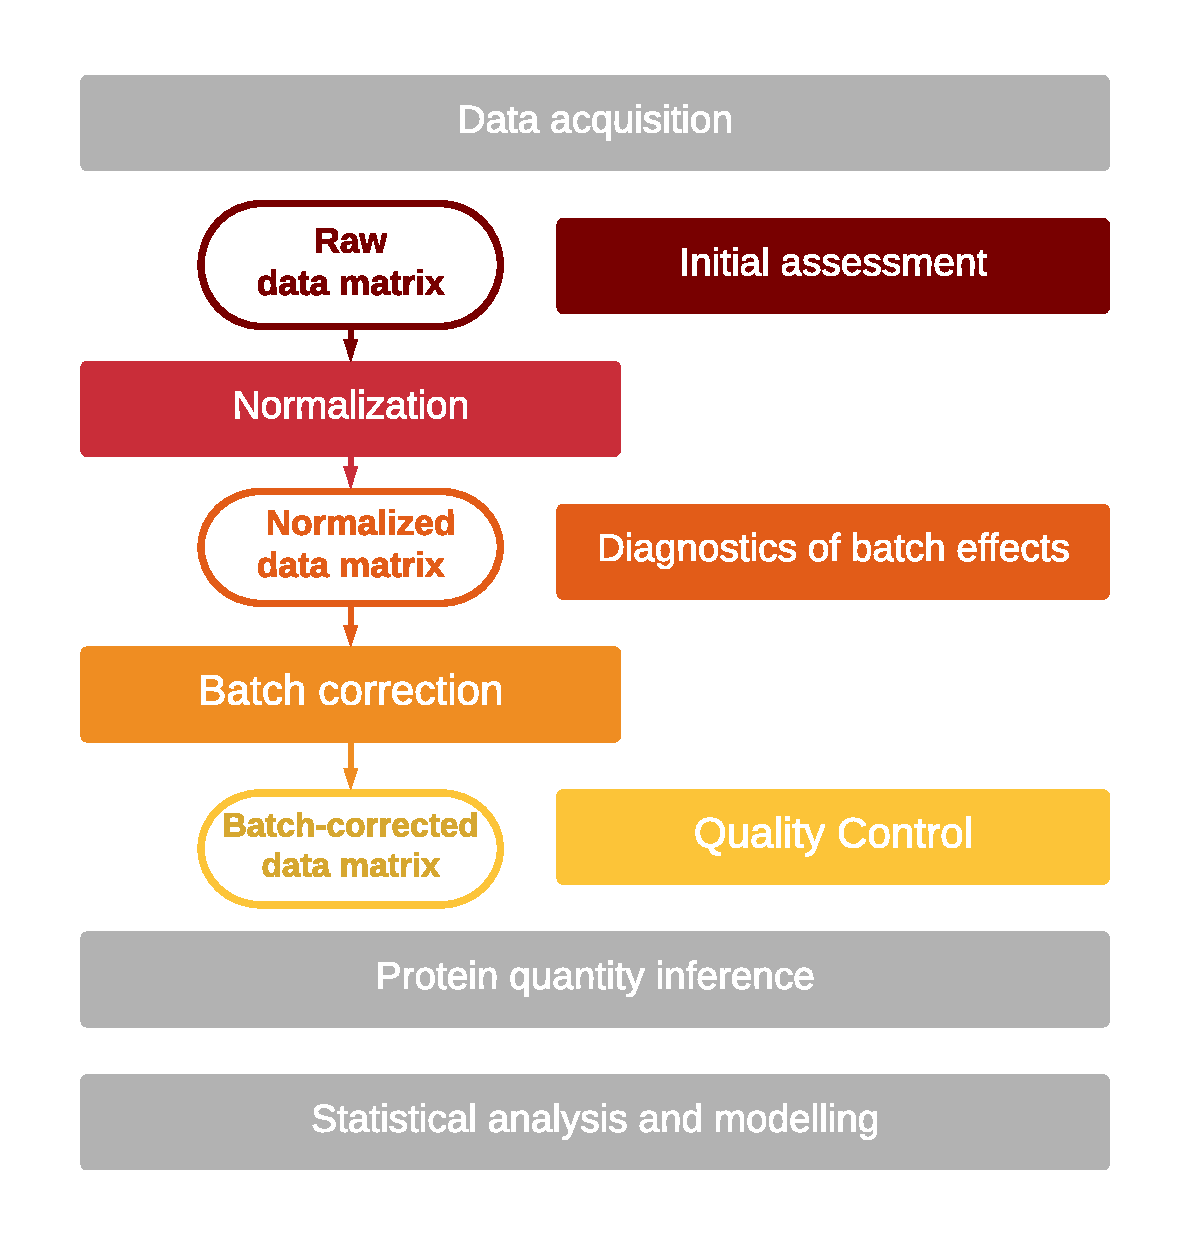
\includegraphics[width=5.1cm]{figures/Fig0_workflow_staircase}
	\vspace{-10pt}
	\caption[Batch effect correction workflow]
{\textbf{Batch effect processing workflow} 

\footnotesize 1. Initial assessment evaluates whether batch effects are present in raw data. 2. Normalization brings all samples from the dataset to the common scale. 3.  Diagnostics of batch effects in normalized data. This step determines whether further correction is required. 4. Batch effects correction addresses feature-specific biases. 5. Quality control tests whether bias has been reduced while retaining meaningful signal.
}
	\label{fig:batch_fig1_workflow}
\end{figure}

In the context of this manuscript, we will use the term “adjust for batch effects” when referring to the whole workflow, and “correct for batch effects” when referring to the correction of normalized data (see \textbf{\hyperref[box:Box1_definitions]{Box 1 "Terminology"}}). 

We provide a checklist that summarizes the most important points of the protocol in \textbf{\hyperref[box:Box2_checklist]{Box 2 "Batch effects processing checklist"}}.
It is also important to stress that batch factors should be considered in the experimental design phase, to ensure that the data are not biased beyond repair, which happens, when biological groups are completely confounded with sample preparation batches  \cite{Hu2005, Gilad2015}. For an extensive discussion of experimental design we refer the reader to previously published materials on the topic \cite{Oberg2009, Cuklina2020}. In this manuscript we assume that experiment was designed with appropriate randomization and blocking, ensuring the correctability of bias, caused by batch effects.

In the accompanying “proBatch” package we implemented several methods with proven utility in batch effects analysis and adjustment. We also provide tips for integrating other tools that might be useful in this context and we provide tips for making them compatible. Extensive comparison of various methods has been published previously \cite{Chawade:2014aa, Luo2010} and here we summarize the best practices from these papers, as well as reviews \cite{Lazar:2013aa, Leek:2010aa}  and application papers \cite{Sajic2018, Collins2017}, and turn them into principles that can guide the reader in choosing an appropriate methodology. 

\subsection{Data matrix before adjustment: choosing between protein-, peptide- and fragment-level input data}
This workflow starts with a raw data matrix, for which initial steps such as peptide-spectrum matching, quantification, and FDR control have been completed. Data are assumed to be log-transformed, unless the variance stabilizing transformation \cite{Durbin2002} is used. In the latter case, the data transformation is included into the normalization procedure. 

We suggest to perform batch affect adjustment on the peptide or fragment ion level, as this procedure alters feature abundances that are critical for protein quantity inference \cite{Clough:2012aa, Teo:2015aa}.  

We also suggest that all detected peptides, including non-proteotypic peptide and peptides with missed cleavages, should be kept into consideration during batch effects adjustment. Keeping all measurements allows to better evaluate the intensity distribution within each sample, which is critical for subsequent normalization and correction steps.

\subsection{Initial assessment}
The goals of the initial assessment phase are to determine bias magnitude and sources, and to select a normalization method.

In most cases, the intensity distributions of samples are different from each other. Comparing global quantitative properties such as sample medians or standard deviations helps with the choice of normalization methods and the identification of technical factors requiring further control. 

Three approaches are particularly useful for initial assessment: 1) plotting the sample intensity average or median in order of MS measurement or technical batch, allows to estimate MS drift or discrete bias in each batch; 2) boxplots allow to assess sample variance and outliers; 3) Inter- vs. intra-batch sample correlation. A higher correlation of samples from the same batch compared to unrelated batches is a clear sign of bias. Optionally, a few proteins or peptides can be checked to see if their quantitative behavior agrees with previous studies or shows signs of bias.



\begin{table}[hbt]
	\begin{tcolorbox}
		\section*{Box 2: Batch effects processing checklist}
		\label{box:Box2_checklist}
		\begin{tabular}{>{\raggedright}p{2cm}m{10.5cm}}
			\headrow
			\thead{Step} & \thead{Substeps} \\
			Experimental design \footnote{For more details on experimental design see \cite{Cuklina2020})}  & \vspace{3 mm}\begin{enumerate}
				
				\item Randomize samples in a balanced manner to prevent confounding of biological factors with batches (technical factors).
				\item Consider adding replicates if possible, for example: a) add replication for each technical factor; b) inject a sample mix every 10-15 samples for control)
				\item Record all technical factors, both plannable and occurring unexpectedly 
			\end{enumerate} \\ 
			Initial assessment	& \begin{enumerate}
				
				\item Check whether the sample intensity distributions are consistent. 
				\item Check the correlation of all sample pairs
				\item If intensities or sample correlation differ, check whether the intensities show batch-specific biases
			\end{enumerate} \\
		
			Normalization		& \begin{enumerate}
				
				\item Choose a normalization procedure, appropriate for biological background and data properties;
				\item Check whether the sample intensity distributions are now comparable (e.g. with boxplots).

			\end{enumerate} \\ 
			Diagnostics		& \begin{enumerate}
				
				\item Using diagnostic tools, determine, whether batch effects persist in the data. 
				\item Use quality control already at this step and skip the correction if it is not necessary.
				\item \textbf{Stopping criterion:} If the goal is to determine differentially expressed proteins, and the batch effects are discrete or linear, multi-factor ANOVA on normalized data is a sound statistical approach. This will adjust for batch effects while simultaneously identifying differentially expressed proteins. This is true even if diagnostic tools indicate the presence of batch effects.
				
			\end{enumerate} \\ 
			Batch effects correction	& 	\begin{enumerate}
				\item	Choose batch effects correction procedure, appropriate for the biological background and data properties, especially those detected at the previous step.
			\item	Repeat the diagnostic step.
			\item	Assess the ultimate benefit with quality control.
\end{enumerate} \\ 

			Quality control 	& 	\begin{enumerate}
				
				\item	Compare correlation of samples within and between the batches. Pay special attention to replicate correlation, if these are available;
				\item	Compare correlation of peptides within and between the proteins.	
			\end{enumerate} \\ 
		\end{tabular}
		
%\footnotetext[1]{For more details on experimental design see \cite{Cuklina2020})} 
	\end{tcolorbox}
\end{table}
\clearpage

\subsection{Normalization}

The goal of normalization is to bring all samples to the same scale to make them comparable. Commonly used methods of normalization are quantile normalization, median normalization and z-transformation. Two main considerations drive the choice of normalization method: 

\begin{itemize}
    \item \textbf{Heterogeneity of the data: }if samples are fairly similar, the bulk of the proteome does not change and thus techniques such as quantile normalization \cite{Bolstad2003} can be used. In datasets in which the samples are substantially different (i.e. when a large fraction of the variables are either positively or negatively affected by the treatment) different methods, such as HMM-assisted normalization can be used \cite{Landfors2011}. Additionally, if some samples are expected to have informative outliers (e.g. muscle tissue, in which a handful of proteins are several orders of magnitude more abundant than the rest of the proteome), methods that keep the relationship of outliers to the bulk proteome, need to be used \cite{Wang770115}.

    \item \textbf{Distribution of sample intensities: }The initial assessment step, especially boxplots, indicate, which level of correction is required: in most cases, shifting the means or medians is enough, but when variances differ substantially, these need to be brought to the same scale as well.
\end{itemize}
It should be noted that after normalization no further data correction might be required. This can be determined with the diagnostic plots and quality control methods, described below. If the results are satisfactory, keeping data manipulation minimal is advisable.

\subsection{Diagnostics of normalized data}
While normalization makes the samples more comparable, it only aligns their global patterns. Therefore, batch effects affecting specific proteins or protein groups might still represent a major source of variance even after normalization. Thus, diagnosis of batch effects is most informative when performed on normalized data. 

The diagnostic approaches can be divided in proteome-wide and peptide-level approaches. The main approaches for \textbf{proteome-wide diagnostics} are:
\begin{itemize}
	\item \textbf{Hierarchical clustering} is an algorithm that groups similar samples into a tree-like structure called dendrogram. Similar samples cluster together and the driving cause of this similarity can be visualized by coloring the leaves of the dendrogram by technical and biological factors. Hierarchical clustering is often combined with a heatmap, mapping quantitative values in the data matrix to colors which in turn facilitates the assessment of patterns in the dataset.
	\item \textbf{Principal Component Analysis (PCA)} is a technique that identifies the leading directions of variation, known as principal components. The projection of data on two components  visualizes sample proximity. This technique is particularly convenient to assess clustering by biological and technical factors, or to check replicate similarity (visualisation without sample point or label overlayment effects works in our experience up to about 50-100 sample in a dataset).
\end{itemize}

One should be careful, however, in interpreting proteome-wide diagnostics because these methods were designed for data matrices without missing values. Proteomic datasets generally contain missing values for technical or biological reasons. For more details, we refer the reader to \textbf{\hyperref[box:Box3_missingness]{Box 3 "Missing values"}}.



In proteomics \textbf{peptide-level diagnostics} are as useful as proteome-wide diagnostic. As in other high-throughput measurements, individual features, in this case peptides, are visualized to check for batch-related bias. In proteomic datasets, spike-in proteins or peptides can be added as controls and used for this purpose. In most DIA datasets iRT peptides \cite{Escher:2012aa}, if added in precise concentrations, are very well suited for individual feature diagnostics.
It should be noted, however, that any random peptide should not be biased in a batch-related manner, so checking a handful of endogenous peptides can also be informative.

Another reason to check individual peptides in proteomics is to examine the trends associated with sample running order. These trends might occur as MS signal deteriorates and require special correction approaches.

Note, that in proteomics, individual features are sometimes not peptides, but transitions or peptide groups. Thus, methods referred here as \textbf{peptide-level diagnostics} are applicable to any feature-level diagnostics.

\subsection{Batch effect correction}

Diagnostics help to determine whether batch effects correction is needed. As global sample patterns have already been corrected during normalization, batch effects affect specific features and feature groups, and that’s the level on which they need to be corrected.

In proteomic datasets two types of batch effects are frequently encountered, continuous and discrete. If batch effects are continuous, e.g.  manifest as MS signal drift progressing from run to run during the sample measurement process, an order-specific curve needs to be fitted. Such drifts are more likely to occur in studies profiling hundreds of samples. This problem is specific to mass spectrometry and is still relatively new to the community. It can be solved by fitting a curve, such as a LOESS fit, or by using any other continuous algorithm.

In contrast, discrete batch effects manifest as feature-specific shifts of each batch as a whole. Here, methods such as mean and median centering work very well. A more advanced modification of the mean shift is provided by ComBat \cite{Johnson:2007aa}. This tool uses a Bayesian framework which has also been successfully applied to proteomic data \cite{Lee:2019aa}. However, ComBat requires that all features are represented in each of the batches. Therefore, especially in large-scale proteomic datasets, applying ComBat might require removal of  a substantial number of peptides that happen to be missing in at least one batch, regardless how small this batch is (see \hyperref[box:Box3_missingness]{Box 3 “Missing values”} for details). Thus, one should be very careful when choosing the method for batch effects correction.

\subsection{Quality Control}\label{subsec:qc}

The purpose of the quality control step is to determine whether the adjustment procedures – normalization and/or batch effects correction – have improved the data. At this step, the data after adjustment are compared to the raw data matrix. There are two types of criteria to evaluate the data quality: 1) Removal of the bias (negative control); 2) Improvement of the data (positive control).

Typically, bias is considered removed if diagnostic plots indicate that similarity between samples is no longer driven by technical factors. This means that neither hierarchical clustering nor PCA show clustering by batch, and correlation of samples from the same batch is no longer stronger than correlation of unrelated samples. Also, individual features should not show batch-related biases. Thus, comparison of diagnostic plots for raw and adjusted data serves as the negative control.

Proving improvement achieved by batch correction is, however, much harder. It is common to take “improved clustering by biological condition” or “higher number of differentially expressed proteins” as a positive control and generally, as a sign of data quality enhancement. However, both criteria can be subjective: it is impossible to know beforehand, whether biological groups are separable in the proteomic space, especially if only a subset of proteins changes and the bulk of the proteome does not. Similarly, it is not possible to predict, whether higher sensitivity for differential expression comes at the expense of added false positive hits. Therefore, we do not recommend using these criteria to assess normalization or batch effects correction. As described above, the choice of the method should rather be based on properties of the samples. However, since batch adjustment removes a certain portion of variance, the coefficient of variation for peptides and proteins in replicated samples should decrease. This is especially true for spike-in peptides or protein that are added to samples in controlled quantities. 

A stronger positive control is assessment of reproducibility. More precisely, one can compare lists of differentially expressed proteins or predictive performance of regression/classification models derived from two or more sample sets belonging to different batches \cite{Lazar:2013aa}. It is expected that in adjusted datasets the resulting lists of differentially expressed proteins, or proteins providing optimal class separation, will be highly overlapping \cite{Shabalin:2008aa}. If two sample sets are independently used for predictive modeling, the predictive performance of such models is also expected to be comparable in adjusted datasets \cite{Luo2010}. Note however, that while this method generalizes well to studies with data acquired by different technologies (e.g. microarrays and RNA-seq for transcriptomics or DIA vs TMT for proteomics), it is restricted to fairly large datasets (several dozens, preferably, hundreds of samples), as predictions from small-scale experiments tend to be unstable.
 
Here we also propose two positive control methods, that do not rely on large sample size and are applicable to most proteomic experiments. The first is based on sample proximity measures, most typically, sample correlation. It is expected, that the correlation of technical or biological replicate samples  is higher than the correlation of unrelated samples. Particularly, the distribution of replicate correlations should be clearly shifted upwards, even though replicates might occasionally correlate less well than some unrelated sample pairs, and this distinction should be strengthened by batch adjustment procedures. Following similar logic, other distance metrics can be used to assess sample proximity, which can also be visualized as improved clustering of replicated samples, seen on hierarchical clustering or PCA component plots. The latter method visualizes every sample in the experiment and thus is most suited to assess studies with up to 150 samples, while bigger sample sizes are harder to visualize.
The second assessment method is specific for bottom-up proteomics, and makes use of peptide correlation. Correlation of unrelated peptides is expected to be close to zero, while peptides originating from the same protein are likely to be positively correlated. Since tens of thousands of peptides are routinely detected in a modern high-throughput proteomic experiment improvements in this metric are a reliable readout of data quality following batch adjustment.

\section{Datasets description}\label{subsec:datasets}

To illustrate the application of the workflow described above, we use two published and one unpublished large-scale proteomic datasets, described in the Table~\ref{tab:batch_datasets}. 

The first study, called here \textbf{"InterLab study"}, assessed the robustness of SWATH-MS in a multi-lab setting \cite{Collins2017}. A set of 30 stable isotope labeled standard (SIS) peptides \cite{Ebhardt2012}, partitioned in five groups, was serially diluted in HEK293 cell lysate. The SIS peptides in the resulting samples spanned a concentration range from 12 amol to 10 pmol. These five sample sets were distributed to 11 laboratories worldwide for measurement by SWATH-MS according to a predetermined schedule. Each of the samples was run on 3 separate days, with the exception of the 4th sample that was run three times on each day. In total, 229 samples were profiled. Thus, the technical covariates whose effect needed to be assessed were the data acquisition site and day. Note that due to the technical nature of the study no biological signal needed to be identified. As only a small number of SIS peptides is different across these samples, all changes can be attributed to technical covariates and therefore the samples in this study can be treated as replicates. Within this manuscript, we analyze only the influence of the acquisition site as a batch factor.

The second study, named here \textbf{"PanCancer study"} \cite{Sajic2018}, profiled the blood plasma glycoproteome of a cohort of patients with five solid carcinomas and matched controls. In total 155 blood plasma samples were collected. Protein digestion and glycopeptide enrichment were performed in 4 batches, several weeks apart. To account for sample preparation reproducibility, 7 biospecimens were replicated and allocated to a different batch. To control for intra-sample variation caused by the sample preparation protocol, bovine fetuin-B was spiked in equal amounts into each plasma sample. In total 162 samples were collected (the validation cohort from the original manuscript is omitted from this analysis).

The third dataset called here \textbf{"Aging mouse study"}, has not yet been published. In this study, the liver proteomes from a BXD reference mouse population \cite{Peirce:2004aa} were profiled to identify proteome changes associated with age. Similarly to prior BXD mice metabolic profiling experiments \cite{Williams:2016aa}, the animals were also subjected to Chow or High-Fat Diet. The samples were randomized with respect to biological covariates (age, diet, sex) and samples from two mice with EarTags "ET1506" and "ET1524" were measured every 10-15 MS runs to control for signal consistency. There are two technical factors affecting the measurement: first, the samples were digested in five batches\footnote{additionally, mix of samples was shot 3 times as control}. Second, to compensate for signal deterioration, MS data acquisition was interrupted for machine cleaning and tuning, resulting in 7 mass-spectrometry batches. These are shown as vertical lines in Figure~\ref{fig:batch_fig2_initAssessment}. As samples were mostly run in the order of digestion batches (see Supplementary figure~\ref{fig:batch_figS3_pipeline_extra}A), the two factors are mostly confounded (i.e. digestion and MS batch mostly overlap). Therefore, in our analysis we only correct for MS batch, unless noted otherwise. Given the particularly severe MS signal deterioration at the end of MS batch 2, the last 13 samples of this batch were profiled again as first samples of MS batch 3. In total, 375 samples are considered in this manuscript.

All in all, these datasets are representative of various applications of large-scale proteomic studies. They make use of various sample sources (i.e. cell cultures, patients and mice). They ask technical and biological questions about proteomes of varying complexity and present different degrees of sample-to-sample heterogeneity. In this respect, the InterLab study is very homogeneous, to the point that all the samples are essentially technical replicates. The PanCancer study is highly heterogeneous, and comprises 205 proteins identified in samples originating from different hospitals and cancer localizations. Finally, the Aging mouse study represent an intermediate case. On one hand, its subjects were genetically very similar and were grown in a controlled environment. On the other hand, sampling from tissues introduced a certain amount of heterogeneity.

\begin{landscape}
	\begin{table}
		\renewcommand*{\arraystretch}{1.8}
		\caption[Dataset description]{Dataset description}
		\label{tab:batch_datasets}
		\small
		\begin{tabular}{|  m{1.75cm}|  m{1.15cm} |  >{\raggedright}m{1.5cm} | >{\raggedright}m{4.13cm} |  m{2.5cm} |  >{\raggedright}m{2.2cm} |  m{1.5cm} |  m{1.5cm} |}
			\hline
			\textbf{Sample} & \textbf{Organism} & \textbf{Sample source} & \textbf{Sample-to-sample heterogeneity} & \textbf{Technical factors} & \textbf{Biological factors} & \textbf{Protein (peak group) number} & \textbf{Number of samples} \\
			\hline
			\hline
			\textbf{InterLab study} & human & cell culture & very low: 
			samples come from the same tissue cultures and differ only by few spike-in peptides
			& \vspace*{1em}\squishlist
			\item data acquisition sites
			\item profiling days
			\squishend
			& --- & 4077
			(31886)
			& 229  \\
			\hline
			\textbf{PanCancer study} & human & blood & high: 
			samples come from cancer patients and matched controls with different cancer localization
			& \squishlist
			\item protein digestion batch
			\squishend
			& \squishlist
			\item case / control
			\item cancer localization
			\squishend
			& 205 (1360)
			& 171  \\
			\hline
			\textbf{Aging mouse study} & mouse & liver tissue & medium: 
			samples come from population of inbred mice originating from two parental strains
			&  \vspace*{1em}\squishlist
			\item protein digestion batch
			\item MS batch
			\item MS drift
			\squishend
			& \squishlist
			\item Strain
			\item Diet
			\item Age
			\squishend
			& 5436
			(33157)\footnotemark
			& 371  \\
			\hline
		\end{tabular}
	\end{table}
	\footnotetext[1]{Number of proteins and peptides before filtering for peptides with too many missing values} 
\end{landscape}

\section{Case Studies}\label{subsec:case_studies}
\subsection{Initial assessment}
The main goal of the initial assessment is to set a baseline for the magnitude and nature of batch effects in a particular data set. At this stage the data matrix is “raw”, the quantities are reported as measured, without any calibration, normalization or correction with regard to their values in other samples.


\begin{figure}[hbt]
	%\center
	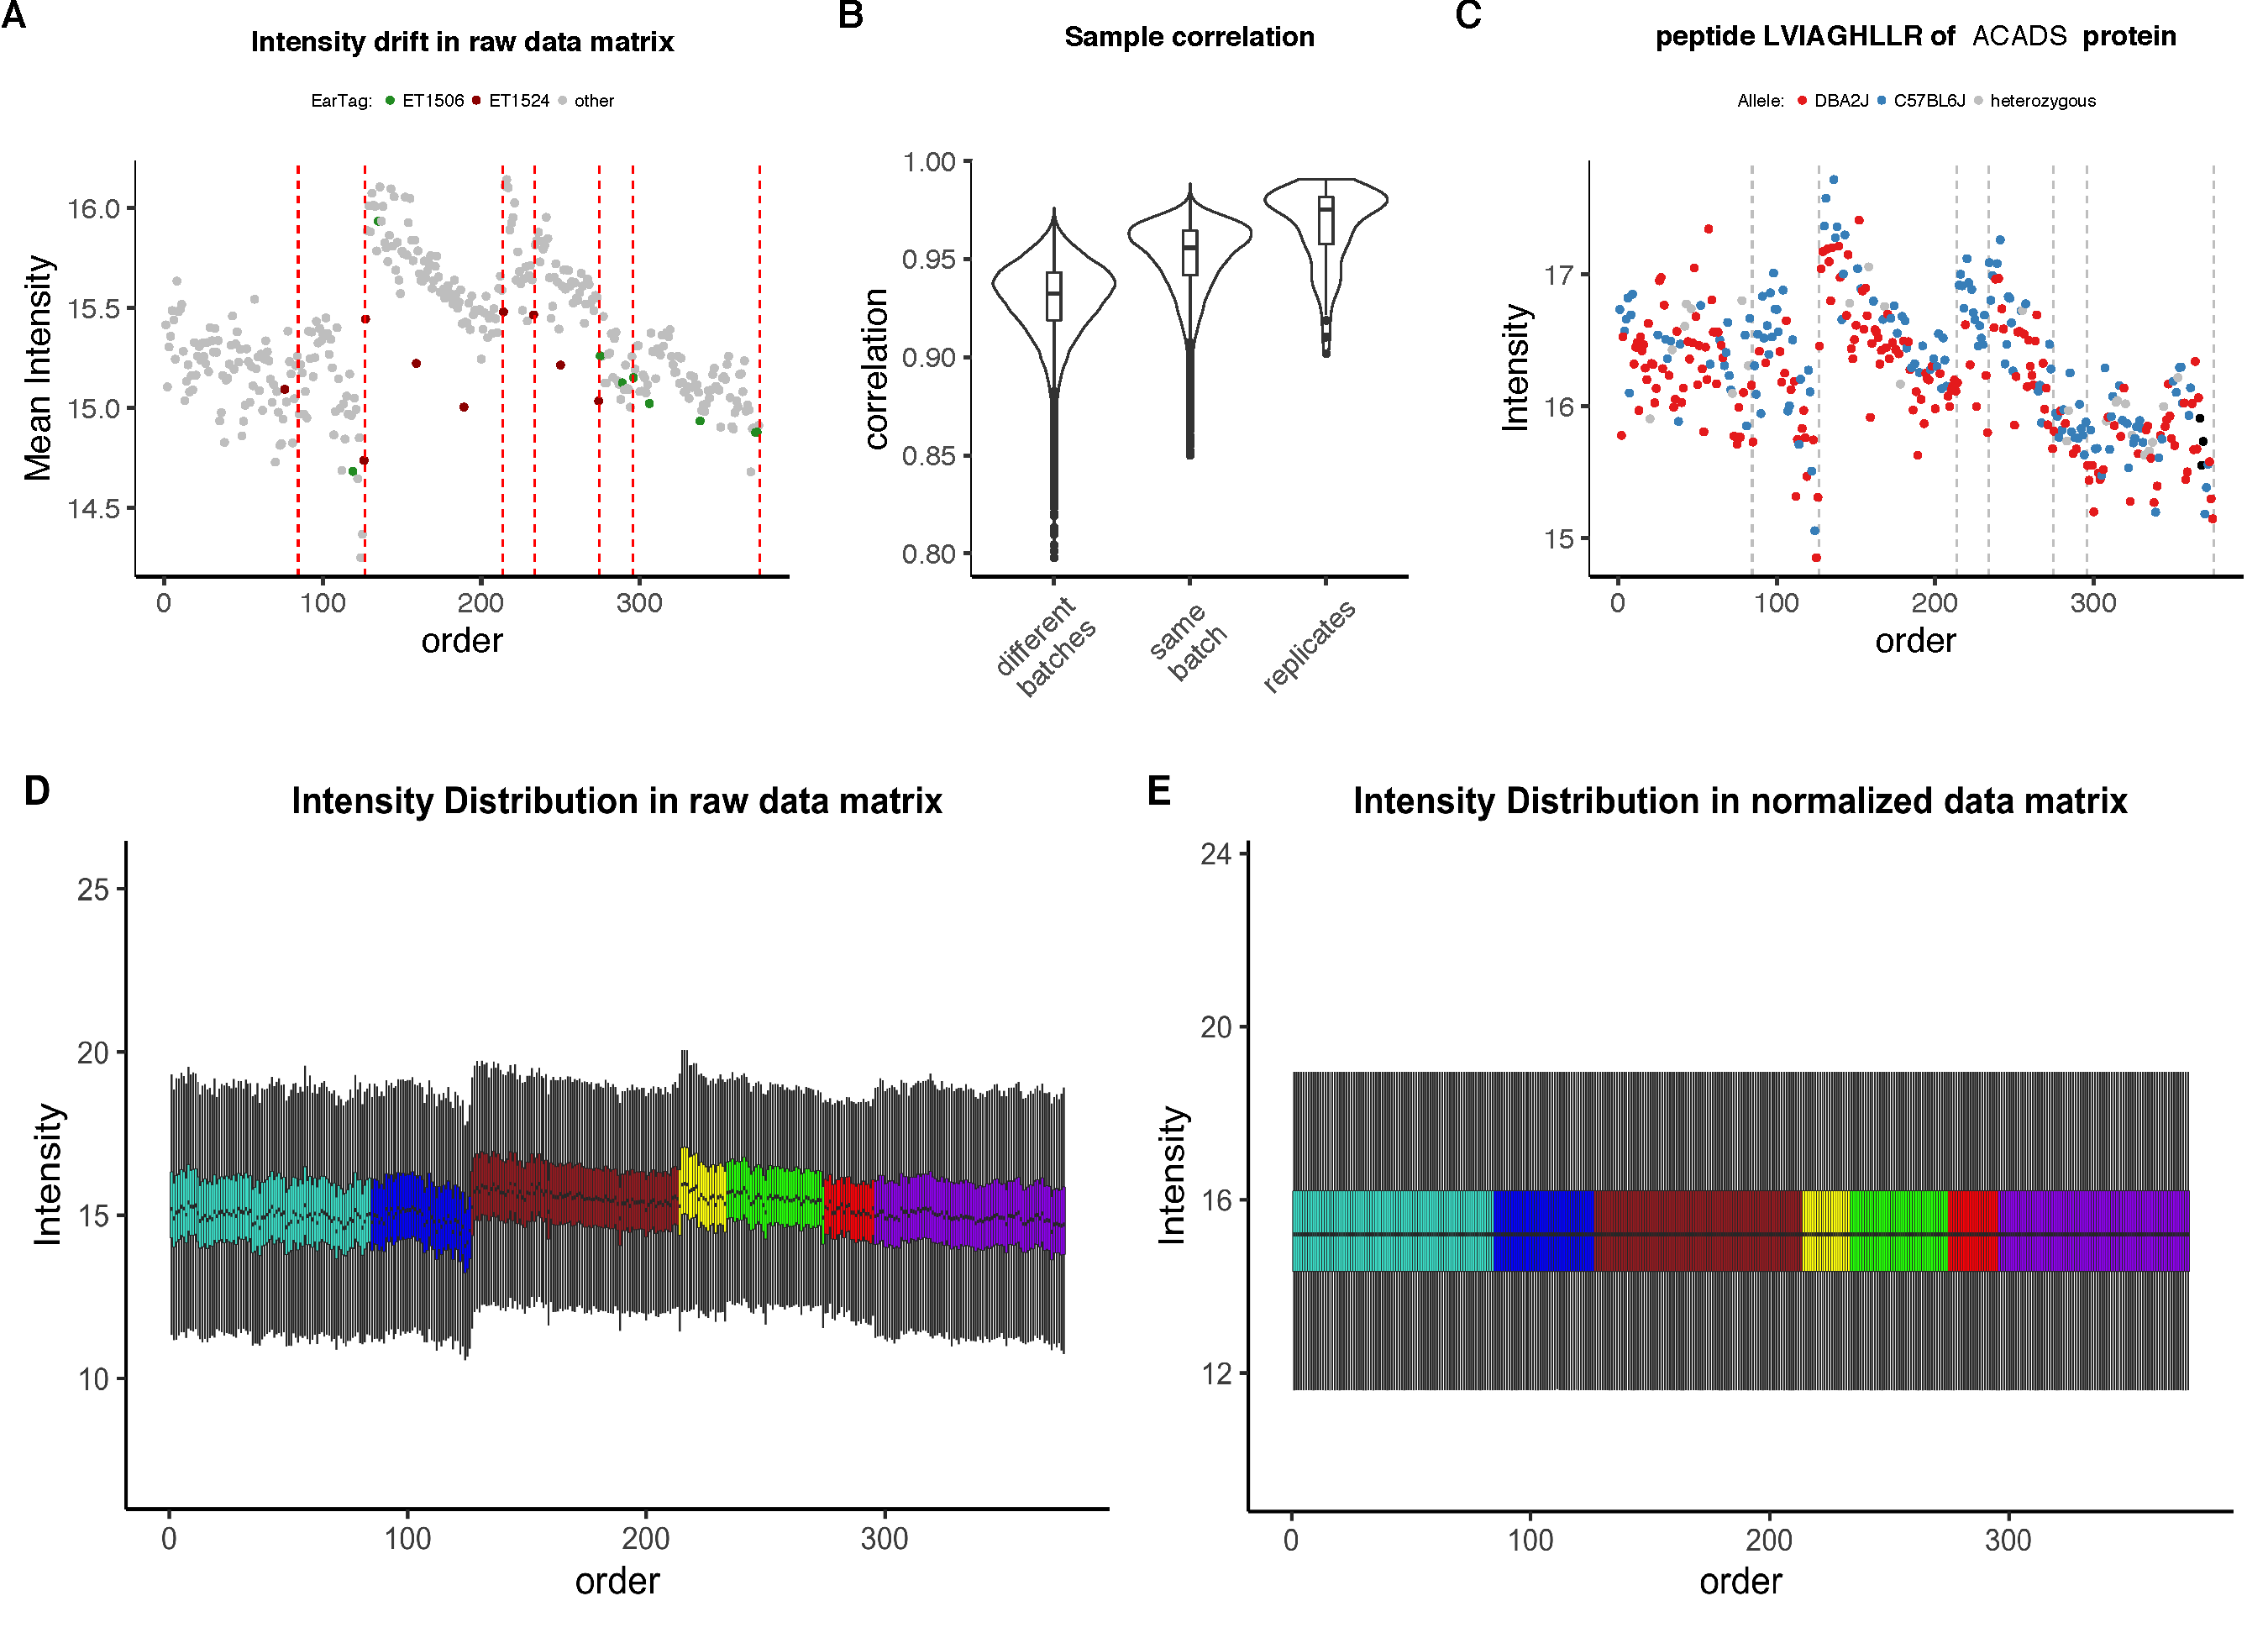
\includegraphics[width=\textwidth]{figures/Fig2_initial_assessment_v1.pdf}
	
	\caption{\textbf{Initial assessment and normalization of the Aging mouse study} \\
		\footnotesize
		(A) Mean Intensity in raw peptide matrix vs sample running order with repeatedly replicated samples shown in color. Vertical dotted lines indicate MS-batch boundaries; (B) Distribution of unadjusted sample intensity correlations - between batches, within batches and in replicated samples; (C) Bias in protein quantification: representative \textit{ACADS} protein, the quantity of which follows the drift of the average sample intensity, preventing allele separation and QTL detection; (D) Boxplots of sample intensities in raw, unnormalized peptide; (E) Boxplots of sample intensities after normalization. All plots represent peptide-level data.}
	\label{fig:batch_fig2_initAssessment}
\end{figure}

Thus, it is essential to get a quick overview of the data by comparing global statistics, such as the average intensity, or correlation, of samples, and of few individual proteins with known expected abundance. In mass-spectrometry, it is important to plot these statistics in a sample running order, as it is common for the measured signal to drift (e.g  due to contamination of the instrument). This is clearly seen in Figure~\ref{fig:batch_fig2_initAssessment}A, where the average intensities of samples from the Aging mouse study are plotted vs the sample running order. In this case, the intensity tended to deteriorate after 50-70 samples. The resulting interruptions for cleaning and calibrating the instrument determined the mass-spectrometry batch. As this type of bias cannot be entirely planned for in advance, it is particularly important to randomize the samples and to include replicates (for more details on sample replication in this dataset see Section~\ref{subsec:datasets} “Dataset description”). 

Not only do batch effects introduce shifts in the total sample intensity distributions, they also lead to spurious correlation between features (i.e. fragments, peptides or proteins). It is common, for samples belonging to the same batch to have strong correlation (as seen in Figure~\ref{fig:batch_fig2_initAssessment}B, Figure~\ref{fig:batch_figS3_pipeline_extra}A, Figure~\ref{fig:batch_figS1_InterLab}B). Often this correlation is not only stronger than the correlation of samples from different batches (“between batches”), but also stronger than the correlation of replicates. Hence, the importance of assessing correlation distributions as early as possible. Sample correlation can be visualized as a square heatmap (Aging Mouse - Figure~\ref{fig:batch_figS3_pipeline_extra}A, InterLab Study -  Figure~\ref{fig:batch_figS1_InterLab}B) or as a correlation distribution box/violinplot (Figure~\ref{fig:batch_fig2_initAssessment}B). The former is preferred with smaller sample sizes (i.e. roughly < 150 samples) and the latter with large datasets, as it is not possible to assess replicate correlation in large datasets on the heatmap.

Optionally, one can complement the initial assessment with the analysis of a few specific features (peptides or proteins), for which prior information is known. In the case study we plot a representative protein \textit{ACADS} with a known quantitative trait locus (QTL), which should be seen as allele separation on the plot. However, as seen in Figure~\ref{fig:batch_fig2_initAssessment}C, the intensity drift, similar to that in Figure~\ref{fig:batch_fig2_initAssessment}A,  prevented the corresponding alleles, descending from strains DBA2J and C75BL6J,  from being separated.

Last but not least, intensity boxplots are extremely powerful at this stage of the analysis, as they visualize in a single plot median, quantiles and outliers. This allows one to see, whether there are batch-specific intensity patterns such as shifts (as in the InterLab study, see Figure~\ref{fig:batch_figS1_InterLab}A), or drifts (as in Figure~\ref{fig:batch_fig2_initAssessment}D), or no evident batch-associated patterns (PanCancer data, Figure~\ref{fig:batch_figS2_PanCancer}A). To detect the patterns, the samples should be sorted by running order or by batch (if the batches, such as digestion batches have been randomized prior to MS analysis). Note that in some cases, intensity patterns might be easier to spot on average intensity plot (compare to Figure~\ref{fig:batch_fig2_initAssessment}A).

\subsection{Normalization}

Normalization is an essential step in removing bias from the data as it brings the samples to the same scale, making the measured quantities comparable \cite{Leek:2010aa}. As stated in Section~\ref{workflow} "Addressing batch effects: the workflow", the choice of normalization method should take two factors into account: 1. heterogeneity, as assessed from previous knowledge, and; 2. global quantitative sample properties, e.g. mean/median/variance, as indicated by initial assessment.

The most common type of normalization, quantile normalization \cite{Bolstad2003}, is applicable to wide a range of samples and was chosen for the Aging mouse data and the PanCancer dataset. As shown in Figure~\ref{fig:batch_fig2_initAssessment}D and E (and Figure~\ref{fig:batch_figS2_PanCancer}A and B), the intensity distributions after quantile normalization are very similar.  This is desirable in experiments where the majority of features are not expected to change, but can be problematic in experimental setups where outliers bear important information \cite{Wang770115}.

Median centering normalization only brings the medians to the same scale and thus is a “milder” approach. This normalization was chosen for the InterLab study and brought the peptide quantities measured at different sites much closer to each other (see Figure~\ref{fig:batch_figS1_InterLab}C). In this dataset, shifting the medians to the same value was sufficient do remove a substantial portion of bias (see Figure~\ref{fig:batch_figS1_InterLab}D, note that the correction on fragment level has residual median discrepancies on protein level). The resulting improvement in signal quality is also reflected in the improved protein quantification precision as illustrated by the reduction in  coefficient of variation for the majority of proteins in the dataset (see Figure~\ref{fig:batch_figS1_InterLab}E).

As shown in this example normalization alone is sometimes the only required correction. In the median normalized InterLab study, the improvement of quantification of spike-in peptides (Figure~\ref{fig:batch_figS1_InterLab}C) and the decrease in protein coefficient of variation (Figure~\ref{fig:batch_figS1_InterLab}E) serve as quality control, and indicate that the further batch correction steps can be skipped.

This is of course not always the case, and batch effects diagnostics should be used, as presented in the next section, to determine if further correction steps are required.


\subsection{Diagnostics}

\begin{figure}[hbt]
	%\center
%	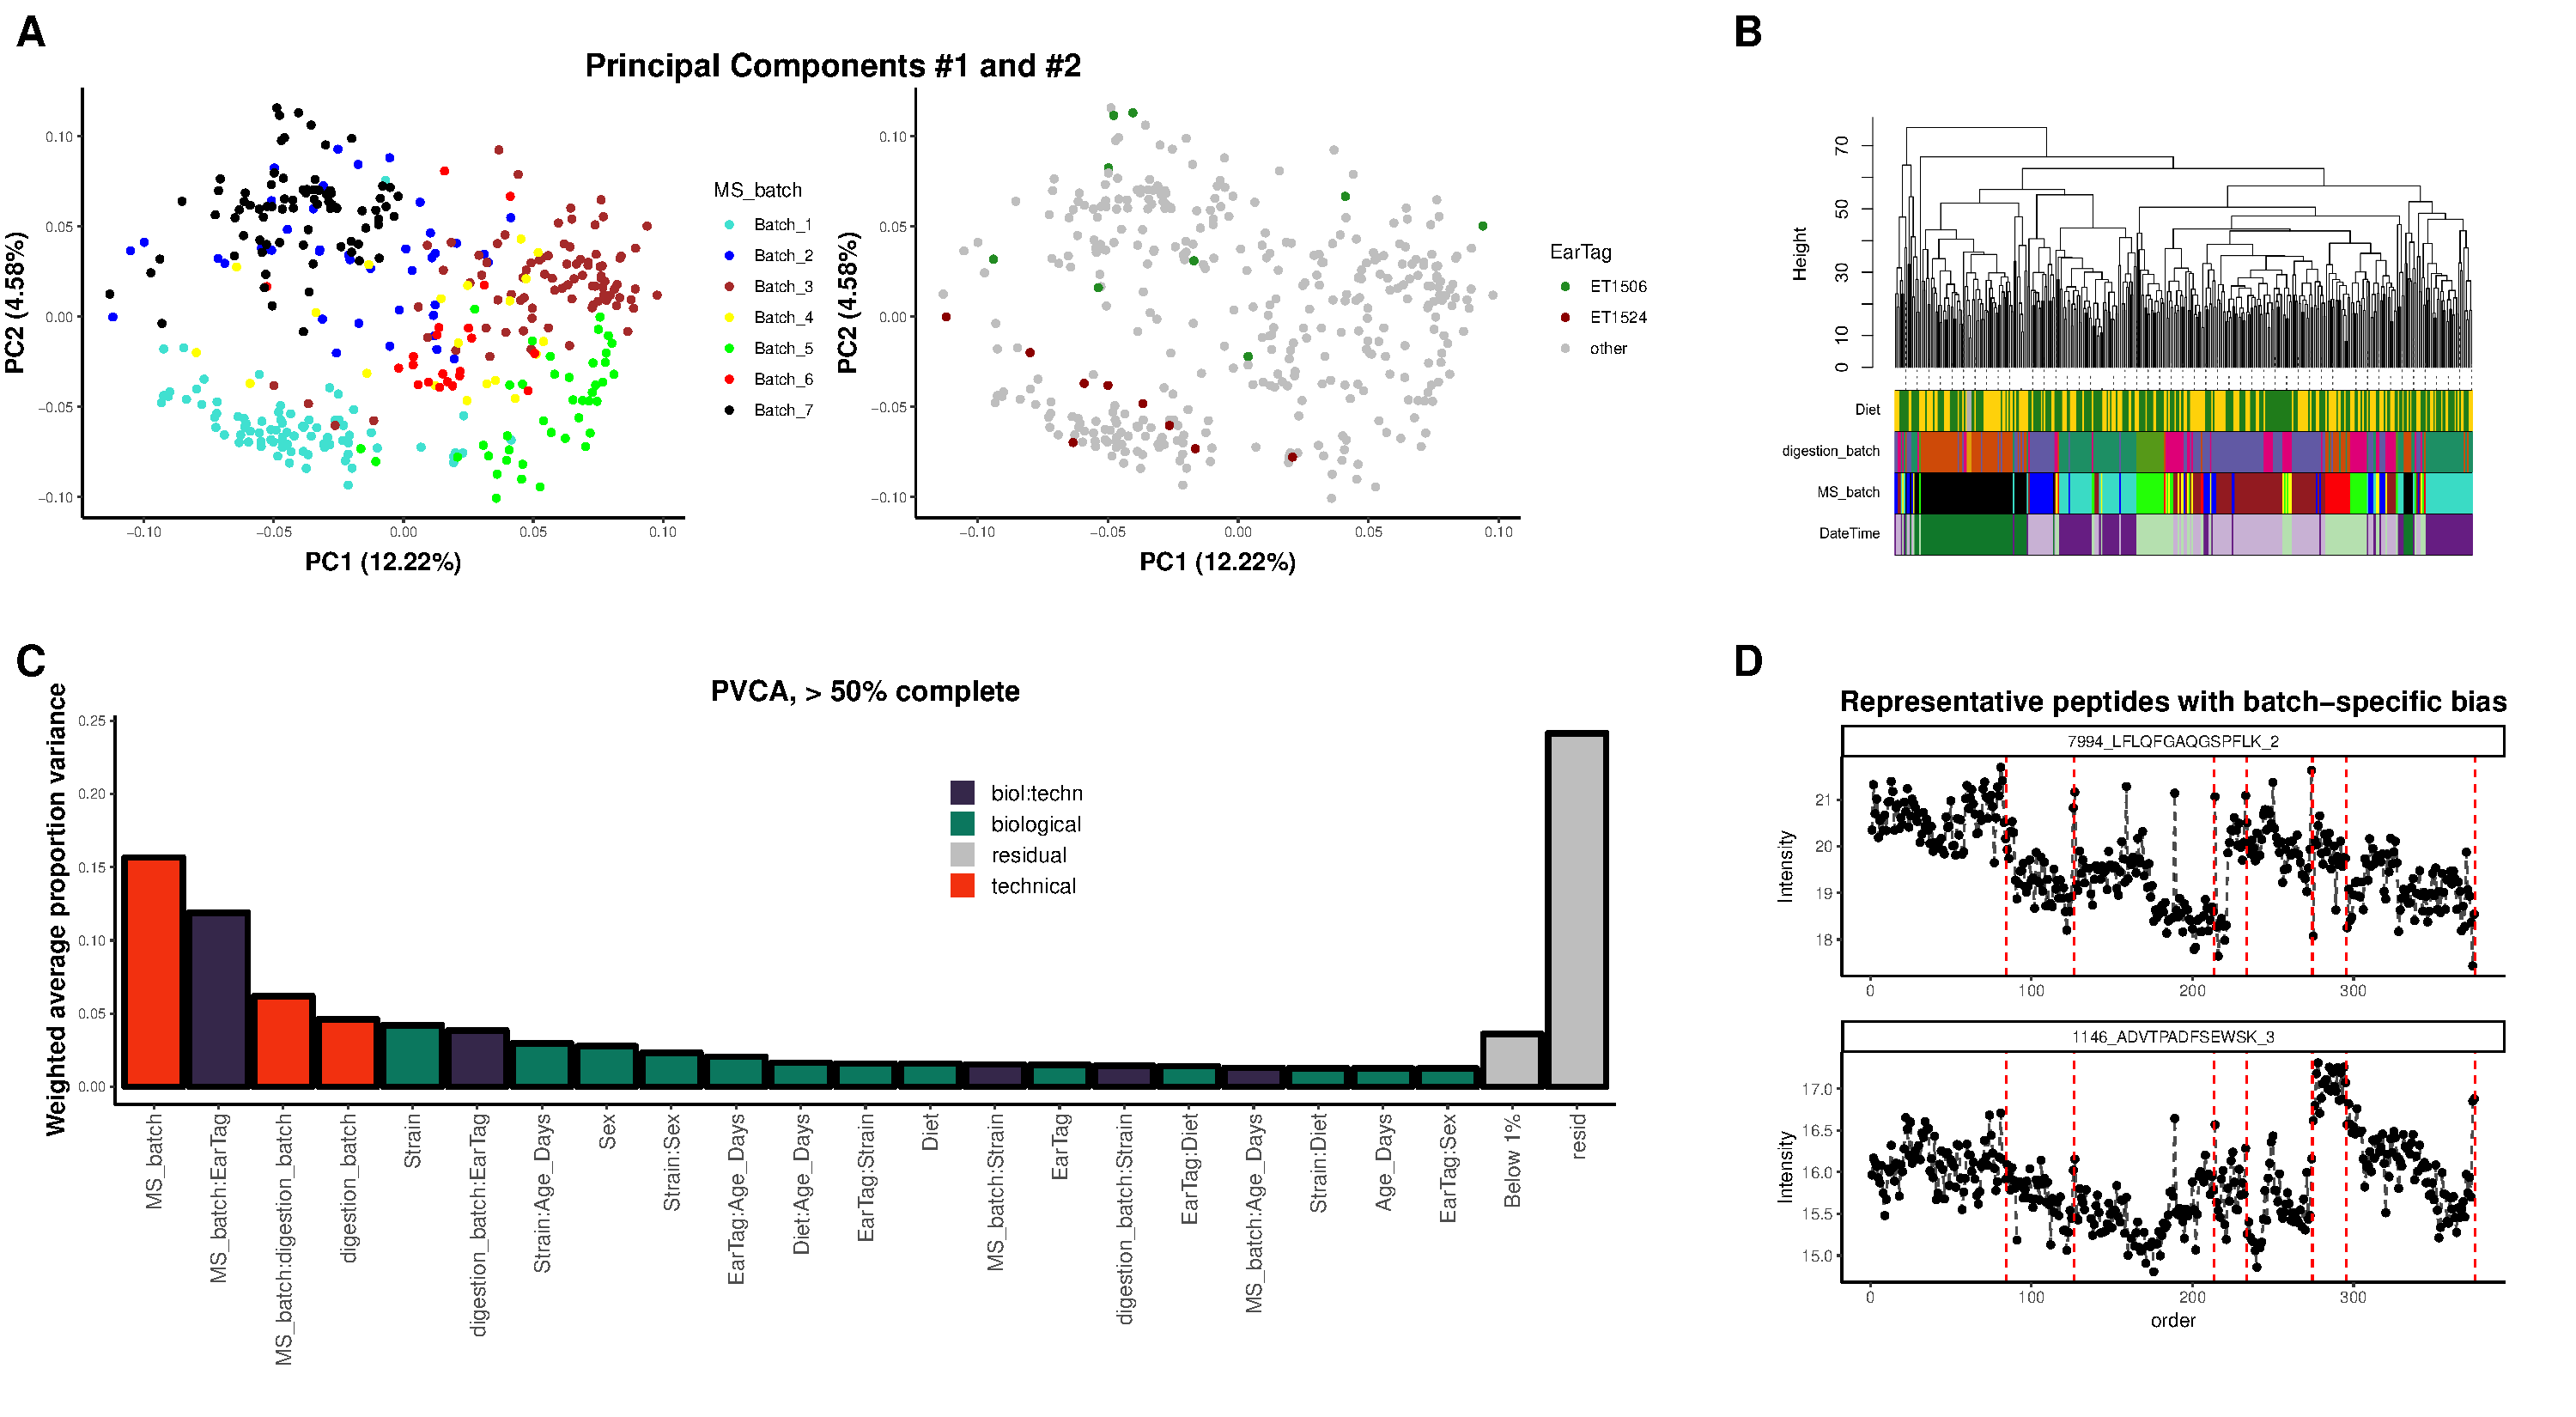
\includegraphics[width=\textwidth]{figures/Fig2_diagnostics.pdf}
	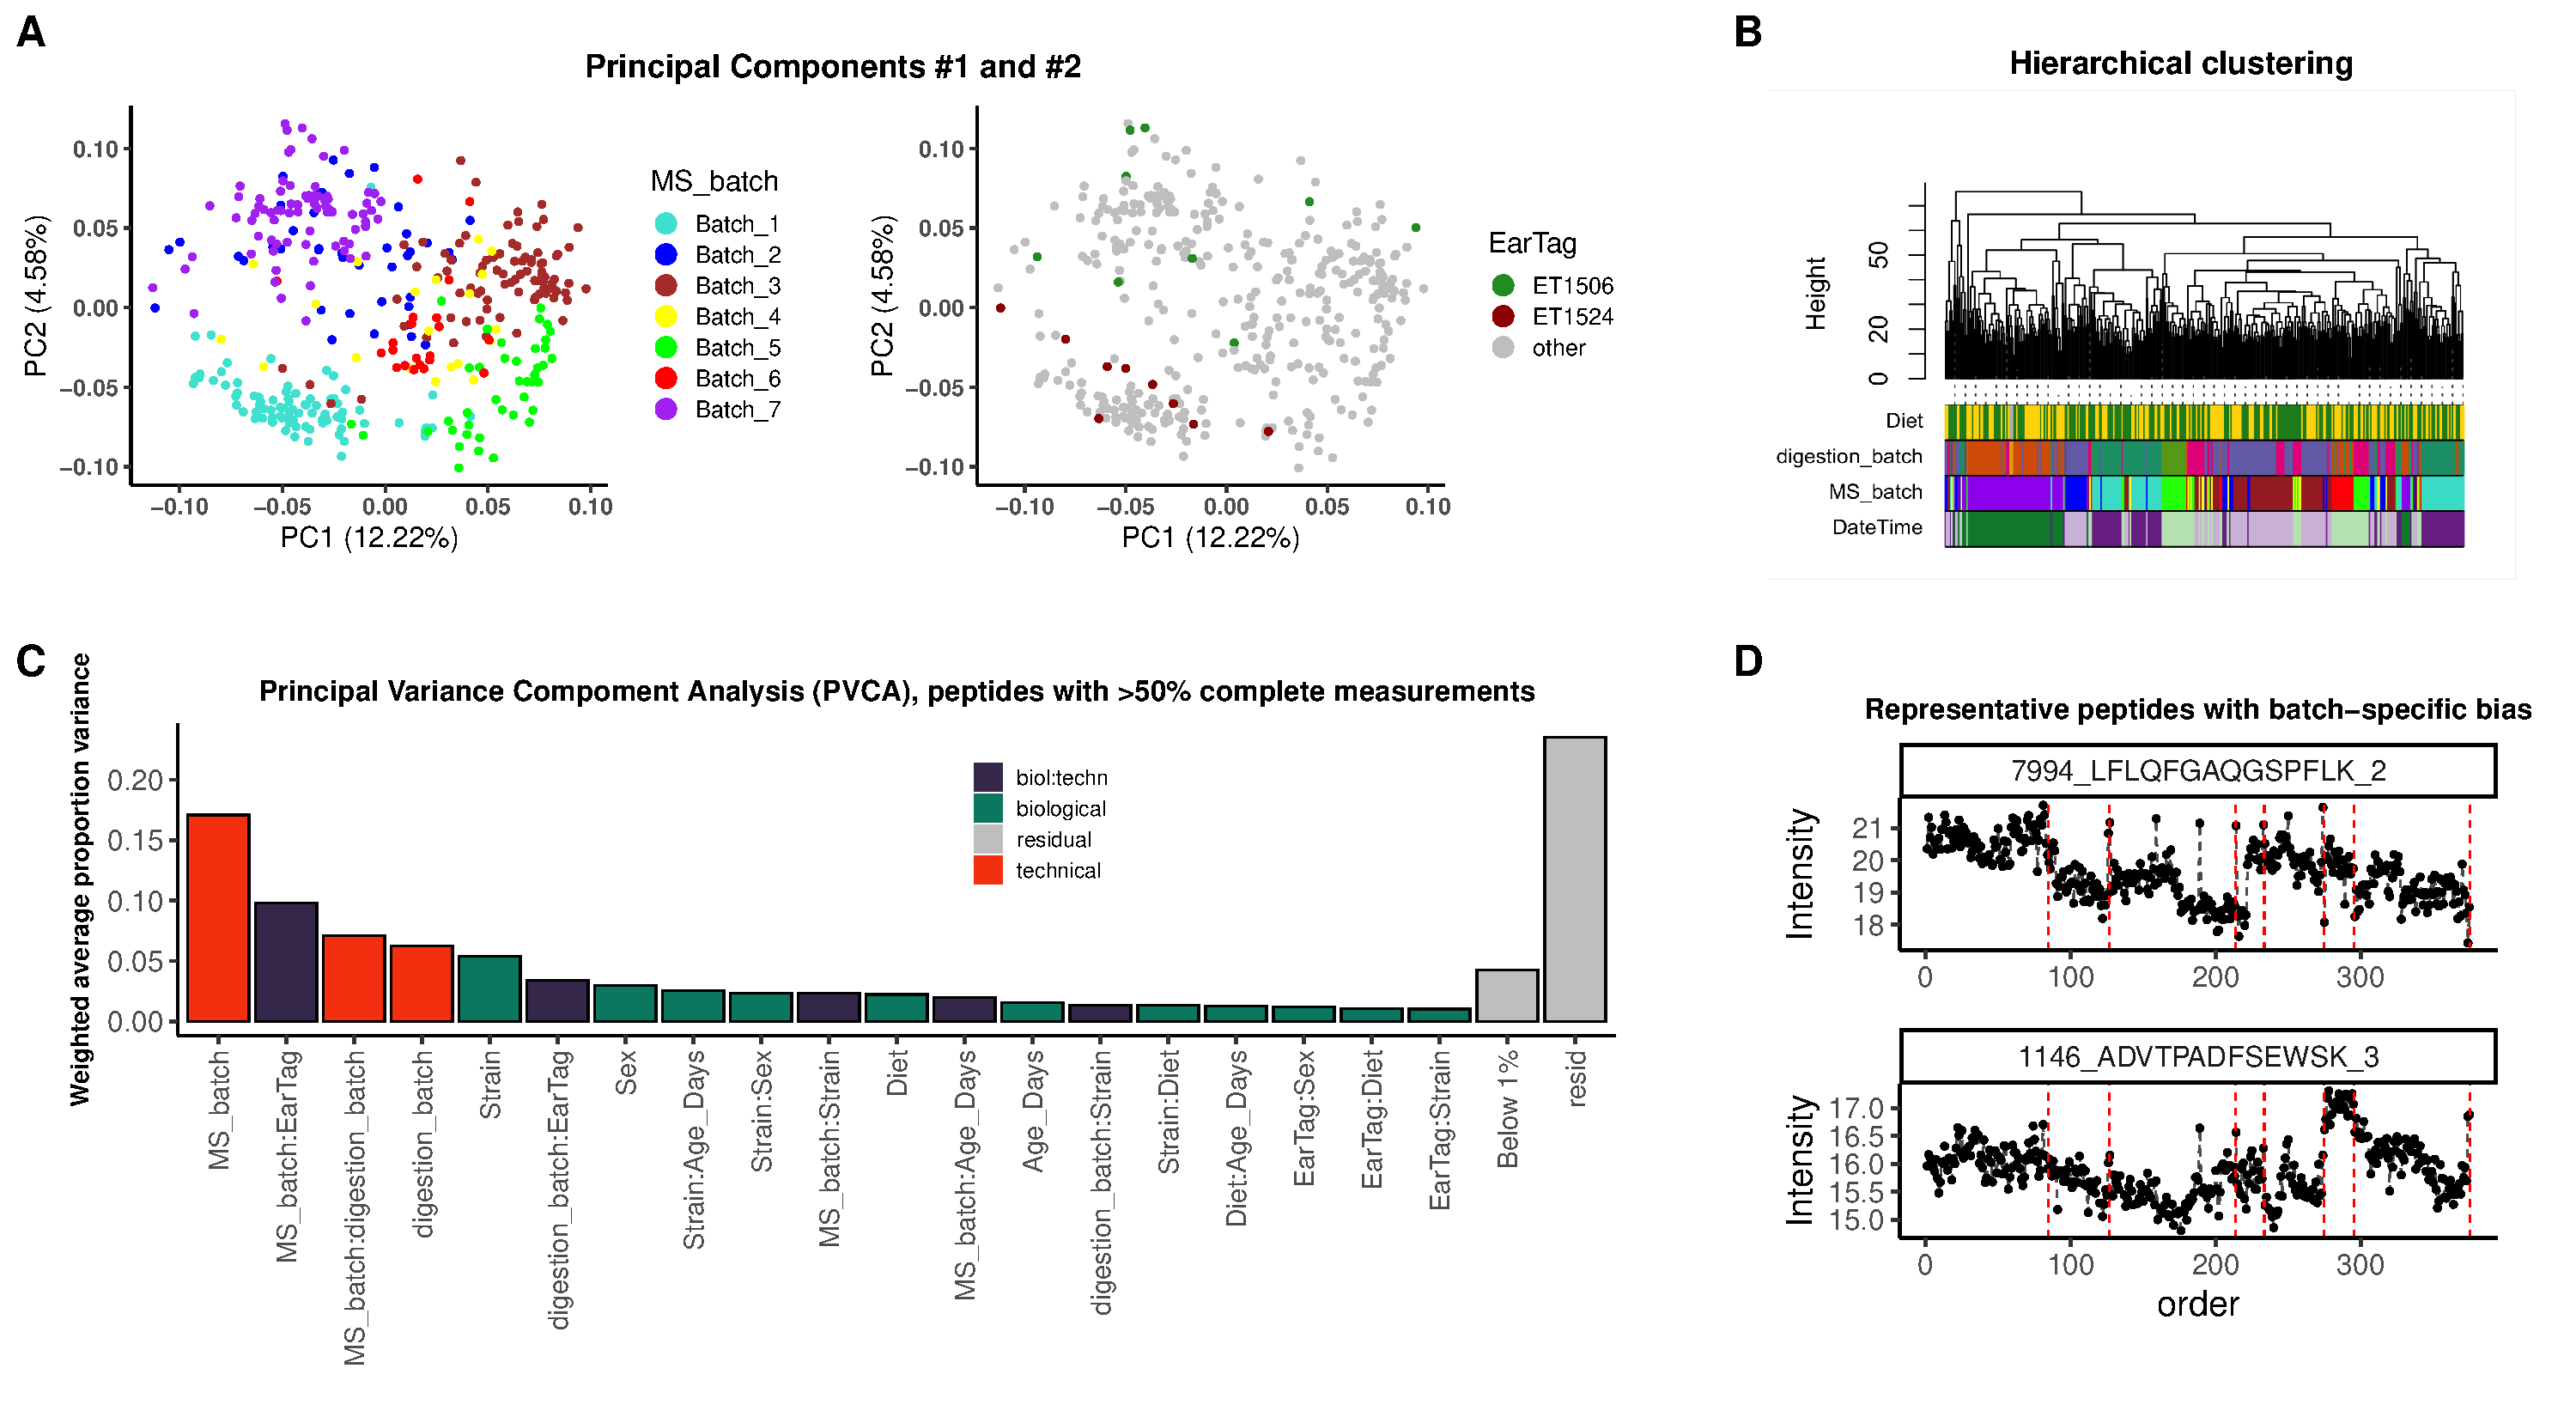
\includegraphics[width=\textwidth]{figures/Fig3_diagnostics1.pdf}
	\caption{\textbf{Diagnostics of batch effects: Aging Mouse study}  \\
		\footnotesize
		(A) Principal Components \#1 and \#2 colored by MS batch (left) and replicates (right). The effect of clustering by MS- batch is dominating, but the replicated samples are closer to each other than just random samples; (B) Hierarchical clustering of samples, with leaves colored by Diet, digestion batch, MS batch and Date-time of sample acquisition is dominated by technical factors; (C) Principal Variance Component Analysis of peptides, detected in >50\% of samples demonstrates, that the technical factors, such as MS batch, digestion batch and their combination has a profound effect on the data, while biological factors such as Strain, Sex and Age account for a much smaller fraction of variance; (D) Peptide-level plots for two iRT peptides demonstrate, that batch effect manifests also as MS signal drift that requires correction}
	\label{fig:batch_fig3_diagnostics}
\end{figure}

Normalization harmonizes overall sample intensities, however, batch effects can still be present at the level of specific features and bias the quantities of many peptides and proteins.
Various methods can be used to assess the extent of remaining bias in the data. Most of them characterize the dataset as a whole, thus working on the proteome level. Methods like Principal Components Analysis (PCA) and Hierarchical Clustering are the best  established. They allow to visualize the factors underlying the similarity of the samples.
Principal Component Analysis is a method that transforms the data matrix into a linear combination of “components” representing the directions of highest variance in the data. This allows high-dimensional data to be visualized in lower dimensions. Additional coloring of the samples by technical/biological factors, or by highlighting replicates, facilitate the interpretation of what drives sample proximity. For instance, in the Aging mouse study, the following patterns became apparent (see Figure~\ref{fig:batch_fig3_diagnostics}A): first, we see a strong clustering of samples by mass spectrometry batch; second, while replicates tend to be close, they are not necessarily the samples with the smallest distance to each other. An overlaid visualization of other factors, such as digestion batch, diet or acquisition date can be found in Figure~\ref{fig:batch_figS3_pipeline_extra}B. 
 
Hierarchical clustering, in contrast, allows one to visualize multiple factors at once (Figure~\ref{fig:batch_fig3_diagnostics}B). Overall, the same patterns identified in the PCA plots are confirmed: clustering is driven primarily by MS and digestion batch, while the effect of diet, a dominant biological factor, is not as strong. Similarly, in the PanCancer study (Figure~\ref{fig:batch_figS2_PanCancer}{C and D, top parts}), we see that the digestion batch is the key clustering factor.

Principal Variance Components Analysis (PVCA) transforms the intuition of visualization brought about by PCA and Hierarchical Clustering into numbers. The weights of each factor in each Principal Component are combined, thus providing a concise summary of variance distribution between biological and technical factors and their combination. In the Aging mouse dataset, we see in Figure~\ref{fig:batch_fig3_diagnostics}C that technical factors such as MS batch, digestion batch, and their combination are leading drivers of variance. Whereas biological factors, such as Diet, Sex, and Age are much less prominent. It should also be noted, that a substantial fraction of variance is “residual”, and cannot be explained by the annotated sample characteristics.

It is important to point out, that most proteome-wide diagnostics rely on data matrices without missing values. Typically for PCA or hierarchical clustering the missing values are imputed (e.g. filled with zeros, small random numbers, or "re-quantified" - filled with summarized MS signal within the projected retention time peak boundaries). However, since missing values are often batch-specific, this might lead to an overestimate of the batch-related clustering and to over-pessimistic assessment of data quality. For more details on the effect of missing values, please refer to \hyperref[box:Box3_missingness]{Box 3 “Missing values”}.

In addition to proteome-wide diagnostics, it is highly advisable to select a few individual features to assess for the presence of feature-level bias. Spike-in peptides and proteins are particularly handy for this type of diagnostics. We illustrate this in the Aging mouse data using iRT peptides, that were spiked at constant quantities in all samples. In Figure~\ref{fig:batch_fig3_diagnostics}D, one can see, that despite the normalization, batch-specific bias still affects the signal. Moreover, this bias is order-related and manifests differently for each of the peptides (for example, in samples 127 – 212 of MS\_batch 3). Also in the PanCancer study, spiked-in Bovine protein Fetuin B quantity is clearly associated with a specific sample preparation batch batch (Figure \ref{fig:batch_figS2_PanCancer} {E}). In contrast to the Aging mouse study here there is no order-related drift, but rather each batch mean is shifted. In conclusion, feature-level bias can be very different in each dataset and checking several representative peptides can help understand the exact nature of the bias.

Together, proteome-level and feature-level diagnostics guide the choice of appropriate batch correction procedure.

\afterpage{%
	\begin{tcolorbox}
		\section*{Box 3: Missing values}
		\label{box:Box3_missingness}
		Proteomic experiments now routinely profile hundreds or thousands of proteins across hundreds of samples. However, detecting all proteins without missing values across the whole dataset is not yet feasible. The patterns of "missingness" are known to be batch-specific \cite{Karpievitch2012}, which is also true for the Aging mouse data (see Figure~\ref{fig:batch_fig4_missing_values} and Figure ~\ref{fig:batch_figS4_missing_values} for details).
		
		It should be noted, that even though "missingness" for low-abundant proteins and peptides is more common than for higher abundant peptides , this problem can also arise due to peptide interference regardless of their abundance. 
        Missing values can also affect batch effects correction methodologies. For instance the current implementation of ComBat \cite{Johnson:2007aa} does not work if a peptide is missing in one batch. One possible solution is to remove all peptides with missing values before the batch correction \cite{Lee:2019aa}. However, this may lead to loss of valuable quantitative information. Thus, methods which are more robust to missing data, such as median-centering, can sometimes be better suited for proteomic data.
		
		Missing values are often imputed, by filling them with zeros, random small values \cite{Tyanova:2016aa} or re-quantification of elution traces \cite{Rost2016}. Such imputation, however, can introduce bias that is batch- or peptide-specific, as seen in  Figure ~\ref{fig:batch_figS4_missing_values}A. In turn, this skews batch effect diagnostic methods, such as hierarchical clustering, PCA or PVCA. In these cases, batch effects assessment will be biased, as the clustering pattern will be driven by missing values Fig~\ref{fig:batch_fig4_missing_values}A. One can estimate this effect by varying the fraction of missing values and assessing to what extent the batch effects are driven by consistently quantified peptides vs missing ones Figure ~\ref{fig:batch_figS4_missing_values}B.
		
		Much more importantly, imputed values may also bias the analysis past the batch effect adjustment stage. As shown in Fig ~\ref{fig:batch_fig4_missing_values}B and C, if "re-quants"   (values inferred from MS elution traces) are used, the correlation within batches seems higher than the correlation of replicates, while this problem is not observed when imputation is not used ("No re-quants"). Protein inference is also affected by the imputation on lower levels.
		
		Finally, provided that there are enough confidently quantified values, many downstream analysis techniques, such as differential expression or protein correlation analyses, can handle missing values. We therefore, advise to avoid imputation, or at least suggest to perform it after batch correction whenever possible. 

		
		\begin{minipage}[h]{\linewidth}
			%\center
			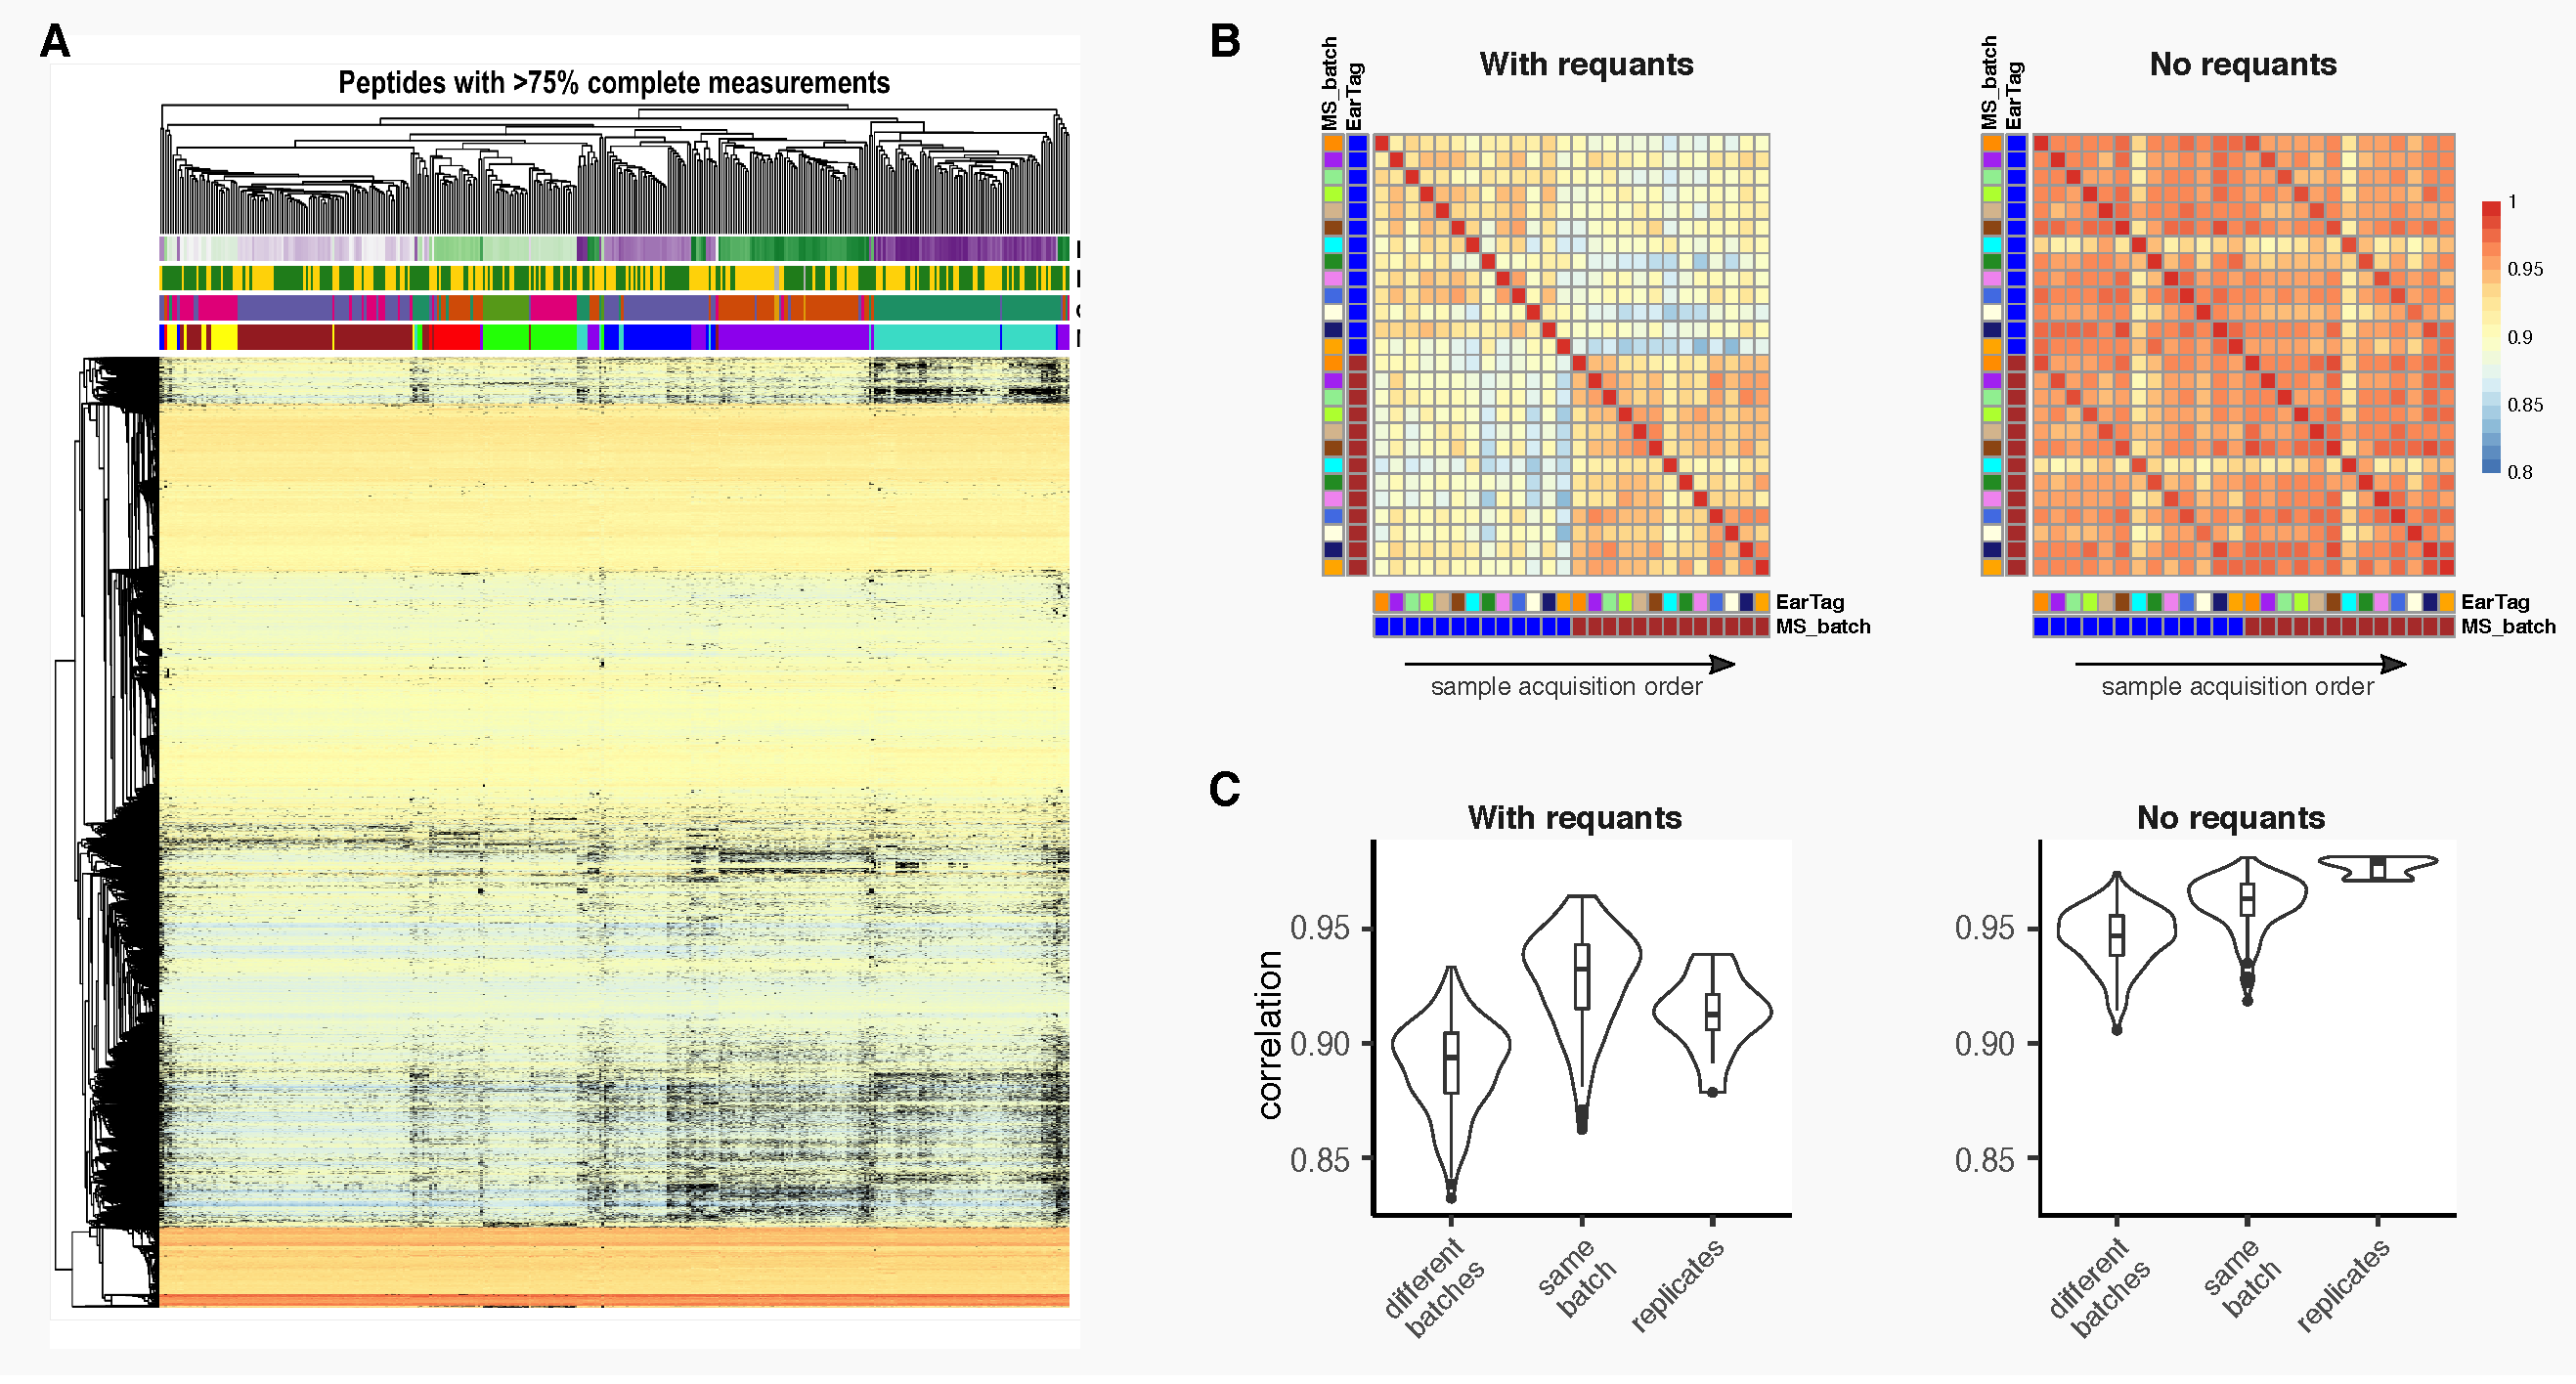
\includegraphics[width=.99\textwidth]{figures/Fig4_missing_values2.pdf}
			\vspace{-.31cm}
			\captionof{figure}[l]{\textbf{The problem of missing values in batch effect diagnosis and correction: Aging mouse study} }
			\label{fig:batch_fig4_missing_values}
			{\footnotesize  (A) Hierarchical clustering of normalized data; Missing values are shown in black. The missing values are non-randomly associated with the batch; (B) Heatmap of selected sample correlation: stronger correlation of samples within Batch 2 (blue) and Batch 3 (brown) is visible in the data with "re-quants", and replicate correlation is much more prominent in the data without "re-quants";	(C) Distribution of selected sample correlation: same effect, as in (B) showing the distribution of sample correlation.}
		\end{minipage}
	\end{tcolorbox}
	\clearpage
}

The goal of batch effects correction is to alleviate the residual bias after normalization. In most cases, normalization significantly reduces the unwanted variance (see representative peptides in Figure~\ref{fig:batch_figS3_pipeline_extra}C), and, as in the InterLab study, might sometimes be the only required adjustment. However, in many cases the batch effects diagnostic procedures described in the previous section will reveal that individual features are differentially affected by batch effects even after normalization (Figure~\ref{fig:batch_fig3_diagnostics}D and Figure~\ref{fig:batch_figS2_PanCancer}C and E). Indeed, batch effects correction is typically applied at the feature-level.

Feature-level bias in proteomics can have different  roots. In the Aging mouse data, the peptides manifest an order-specific, continuous bias, while the PanCancer data exhibits discrete shifts. The latter can be corrected with methods established by the genomics community, whereas the former is typical of large MS-based proteomic experiments and will therefore be discussed in more details in the following paragraphs.

In MS-based proteomics, samples are analyzed sequentially, typically using an on-line chromatographic system directly coupled to a mass spectrometer. Various components of this system are susceptible to degradation of performances over time (e.g. changes in the properties of the chromatographic material, emitter degradation, contamination of MS lenses, mass calibration drift). Various factors, such as sample quality and composition, can contribute to the speed of this degradation. However, even under best conditions, one can expect to see noticeable degradation after a few hundred runs. Therefore, continuous batch effects associated with signal drift are characteristic of MS-based proteomics. They are also increasing in importance as they are particularly relevant in large scale studies. For instance, the Aging mouse study was comprised of almost 400 samples and therefore had to be split into 7 MS measurement batches, each with a unique signal drifting pattern to it.

To address this complex bias, we have developed a two-step batch correction procedure shown in Figure~\ref{fig:batch_fig5_batchCorrection}. In the first step, MS signal drift is corrected based on non-linear curve fitting. As a curve-fitting algorithm, we have chosen LOESS, as it combines computational simplicity with relative flexibility of the fit characteristics. The procedure runs as follows: for each peptide and each batch, a unique curve is fit (Figure~\ref{fig:batch_fig5_batchCorrection}A), and then subtracted from the normalized intensity value in each sample, leading to measurements, whose median is different in each batch (Figure~\ref{fig:batch_fig5_batchCorrection}B). Note, that LOESS has a parameter "span": smaller span fits minute details, while when the span is too big, some of the trends get missed, meaning the each time the span has to be adjusted to each dataset individually (see Figure~\ref{fig:batch_figS3_pipeline_extra}). Alternatively, other algorithms, such as SVM and Random Forest, can be used to correct for the MS signal drift \cite{Luan2018, Shen2016}.   After that, a discrete batch effects correction procedure can be applied (e.g. median centering, ComBat, ...). In the Aging mouse (Figure~\ref{fig:batch_fig5_batchCorrection}C) and PanCancer (Figure~\ref{fig:batch_figS2_PanCancer}C-F) studies we opted to use median centering at this stage. It should be noted that while this approach can cope with missing values, having a significant percentage of missingness will compromise its effectiveness. For more details on missing value problem see \hyperref[box:Box3_missingness]{Box 3 "Missing values"}.

\subsection{Batch effects correction}
\begin{figure}[hbt]
	%\center
	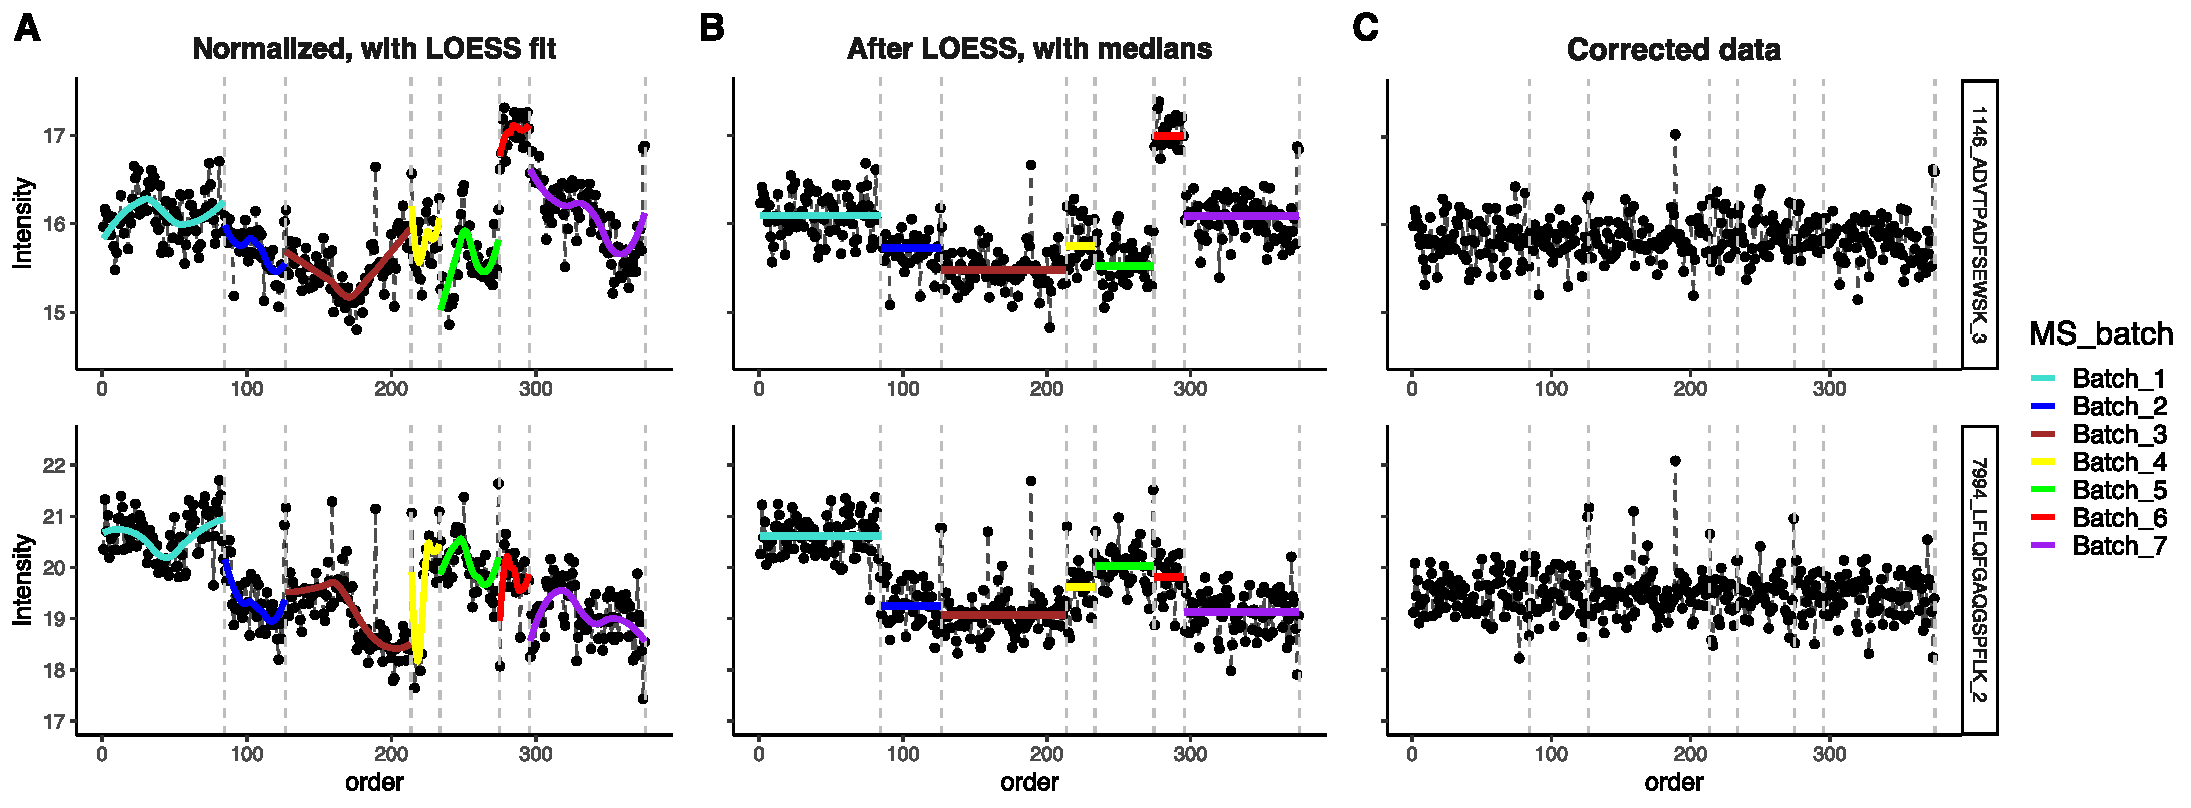
\includegraphics[width=\textwidth]{figures/Fig5_batch_correction1.pdf}
	
	\caption{\textbf{Two-step correction of batch effects}  \\
		\footnotesize
		(A) Fitting a LOESS curve for every peptide in each batch and subtracting the fit; (B) Using medians for correction of the residual discrete batch effect; (C) The corrected data is more uniform and can now be used for downstream analysis. Data from the Aging mouse study.}
	\label{fig:batch_fig5_batchCorrection}
\end{figure}

When several batch factors affect the data (as diagnosed by PCA, Hierarchical clustering and/or PVCA), all factors should be accounted for during correction. This typically means that batch factors get combined. This however, is not always possible. In the Aging mouse study for instance, the two main technical factors, MS batch and digestion batch, were highly confounded. Thus, we opted to only correct for MS batch.

In conclusion, batch effect correction removes variance from known, annotated batch factors. Whether the adjustment procedures – normalization and batch effects correction – improved the data signal, remains however to be determined by a quality control step.


\subsection{Quality Control}
\begin{figure}[hbt]
	%\center
	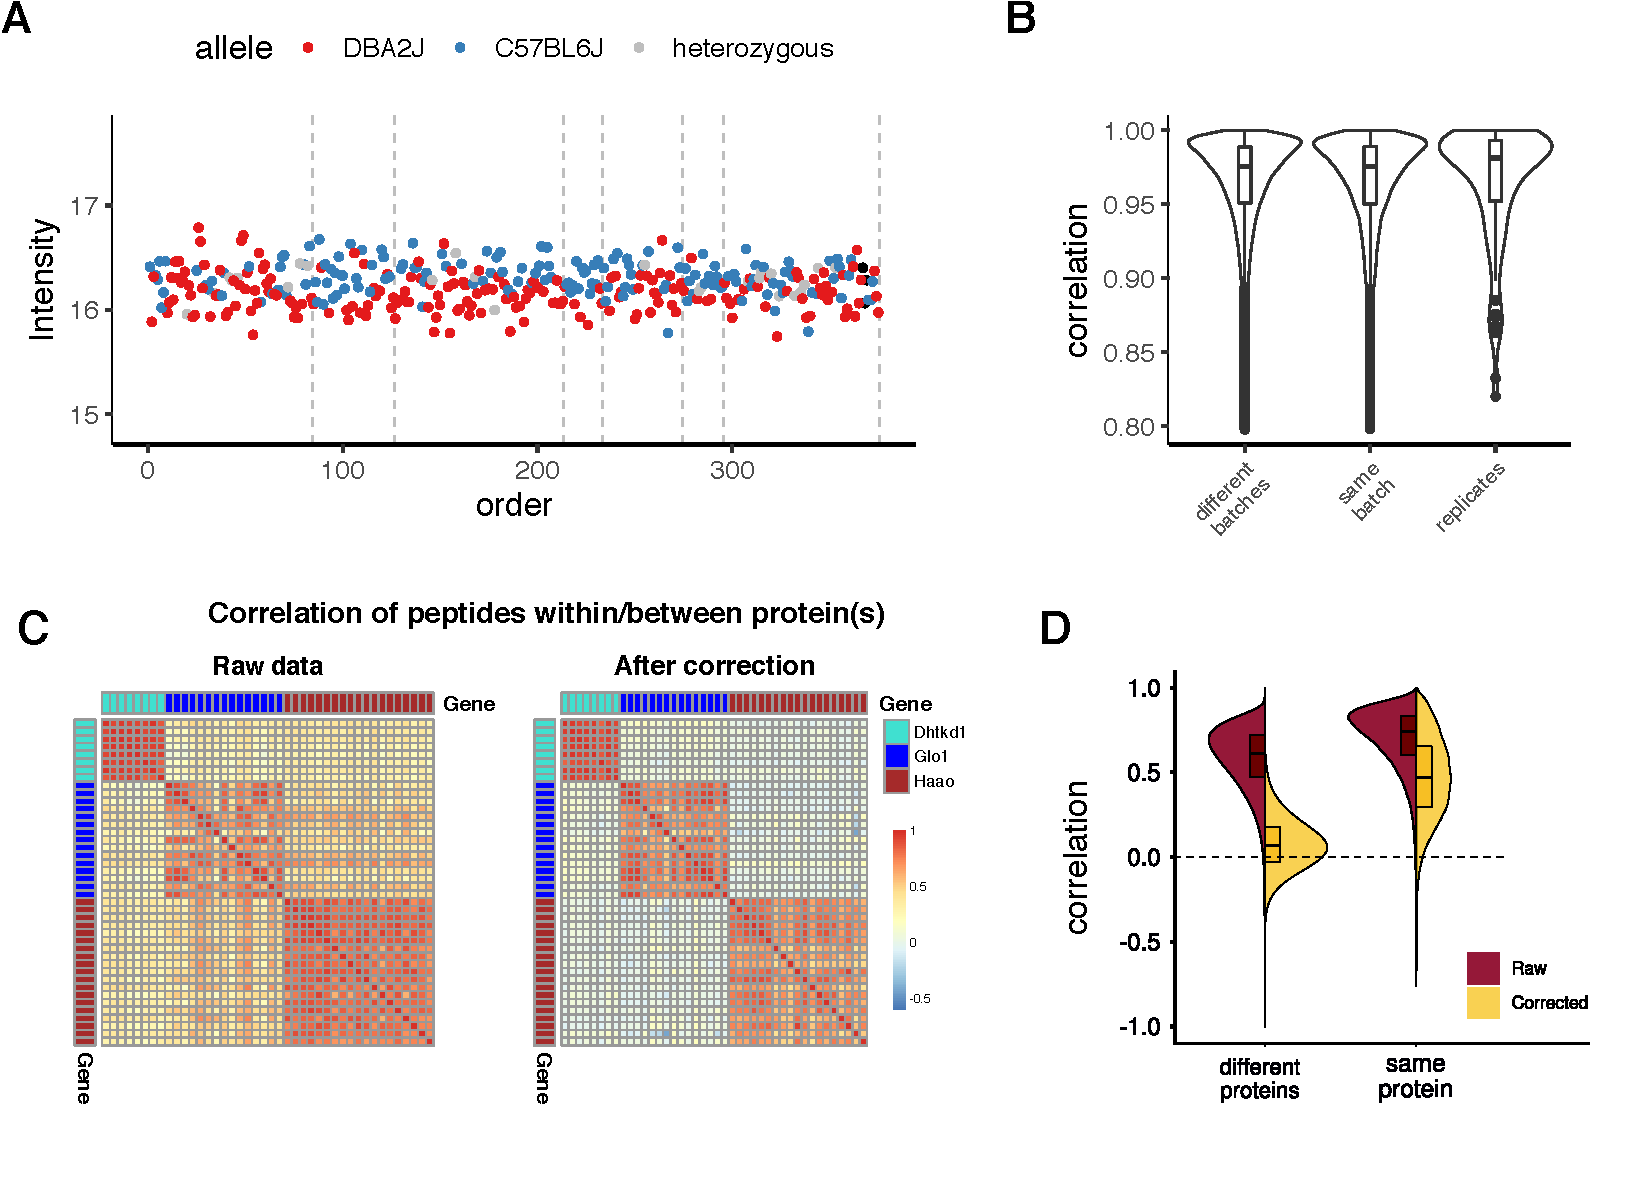
\includegraphics[width=\textwidth]{figures/Fig6_quality_control2.pdf}
	
	\caption{\textbf{Quality control of batch effects correction}  \\
		\footnotesize
		(A) Representative "Acads" protein QTL, that in corrected data demonstrates a clear improvement in allele separation; (B) Distribution of sample correlations - between batches, within batches and in replicated samples for corrected data; (C)  Heatmaps of peptide correlation for the proteins DHTKD1, GLO1 and HAAO, before and after correction: correlation is positive for all peptides in the raw matrix, while after batch correction the correlation of unrelated peptides becomes close to zero; (D) Distribution of peptide correlation in raw data (brown) and in batch corrected data (yellow) for peptides from different proteins and peptides from the same protein: while same-protein peptide correlation is always higher than the correlation of unrelated peptides, the correlation of unrelated peptides approaches zero only after the correction.}
	\label{fig:batch_fig6_QualityControl}
\end{figure}


The main goal of the quality control step is to determine, whether the data quality has improved. 

Examples of negative controls are the plots discussed in the diagnostics section like individual peptides plots, PCA, hierarchical clustering or PVCA. In most cases, these show that samples are no longer affected by batch-specific patterns (e.g. PanCancer study hierarchical clustering in Figure~\ref{fig:batch_figS2_PanCancer}C and D and corrected Bovine Fetuin B protein in Figure~\ref{fig:batch_figS2_PanCancer}E and F and ).

Depending on the experimental setup, one can sometimes judge the data improvement through the presence of better biological signal. In the Aging mouse study, this can be achieved via known protein Quantitative Trait Loci (pQTL), particularly \textit{cis}-QTLs (i.e. alleles of specific genes  affecting protein expression from that locus). As seen in Figure~\ref{fig:batch_fig6_QualityControl}A, certain proteins become clearly easier to separate and less biased than before the bias adjustment (compare to Figure~\ref{fig:batch_fig2_initAssessment}C). As a result, there is a clear increase in pQTL detection sensitivity: 255 pQTLs passed the significance threshold in the raw data matrix, and extra 133 pQTLs have been detected after batch effects adjustment - 100 after normalization and 33 additional pQTLs after batch effects correction. In this case, normalization seems to alleviate the most of the bias, as was already demonstrated in \ref{fig:batch_figS3_pipeline_extra}C. This effect is quite common, and is the reason why the batch effects correction step was not performed in the InterLab study. Skipping batch effects correction is particularly common, when the next analysis step is ANOVA, or it is not clear, which technical factor should be corrected for (e.g. diagnostic plots don't show a clear clustering pattern and the weights of technical factors on PVCA are low).  However, when biological groups are not confounded with technical factors, batch correction usually improves signal and reduces noise.

On the other hand, the sample and feature proximity methods we proposed in Section~\ref{subsec:qc} “Quality control”  can be applied to in almost any proteomic experimental context.

Sample proximity measured as correlation distributions for intrabatch vs. unrelated samples, and for replicates vs. all other samples can be seen for the Aging mouse dataset pre- and post-adjustment in Figure~\ref{fig:batch_fig2_initAssessment}B and Figure~\ref{fig:batch_fig6_QualityControl}B. This approach and considerations can also be applied with different distance measures and visualizations. Figure~\ref{fig:batch_figS2_PanCancer}G and H demonstrate this concept on the PanCancer data using Manhattan distance and a hierarchical clustering representation. These, proximity-based quality controls are universally  applicable to any dataset with replicated samples and batches.

The second method is based on assessing the proximity of feature sets. In bottom-up proteomics these are peptides or fragments. Similarly to the previous method, the distance between related peptides (i.e. belonging to a common protein) is expected to be smaller than the distance between unrelated ones. This effect is true not only for selected proteins (Figure~\ref{fig:batch_fig6_QualityControl}C left) but also holds true for the whole proteome (Figure~\ref{fig:batch_fig6_QualityControl}D, dark brown). The correlation of unrelated peptides, however, gets much closer to zero after the correction (Figure~\ref{fig:batch_fig6_QualityControl}C right, and Figure~\ref{fig:batch_fig6_QualityControl}D yellow). Hence, before batch adjustment most of the peptide correlation was spurious.

In summary, through a combination of positive and negative quality controls, it is possible to assess improvements in data quality. It should however be stressed, that quality control methods are not criteria for choosing batch adjustment methods. Rather their purpose is to provide metrics to control the quality of the data before and after adjustment.

\section{Computational tools and analysis}

To facilitate the practical application of the steps and principles described in this manuscript, we have developed an R package, named "proBatch" and made it available in Bioconductor \url{https://bioconductor.org/packages/release/bioc/html/proBatch.html}. The "proBatch" package wraps multiple established techniques for data transformation and visualization with proven utility in control of batch effects. 

The package has been designed based on the following principles to facilitate the construction of batch effect adjustment pipelines:
\begin{itemize}
    \item For each step of the workflow one or more functions are provided.
    \item The input to each function is standardized to a feature measurement table (e.g. peptide, protein, fragment, transition) and a sample annotation table with technical and biological factors.
    \item Consistent visual representation of factors at all steps of the analysis (e.g. color scheme defined once per analysis).
\end{itemize}

Note that we have also deliberately avoided the inclusion of a "single-click" batch adjustment function, that would combine normalization and correction. We decided on this implementation to promote awareness of the properties of a particular dataset and to enable informed choice of appropriate batch adjustment methods.

We also make the code used for the analyses of the three case studies presented in this manuscript available on GitHub \url{https://github.com/symbioticMe/batch\_effects\_workflow\_code}. An accompanying docker container containing all the tools required to replicate the analyses is made available on Dockerhub (https://hub.docker.com/repository/docker/digitalproteomes/probatch).

\section{Discussion}

The meaningful analysis of data generated by large-scale proteomic studies, made possible by recent technological advances in data collection, is critically dependent on the statistical power required for systems biology and translational medicine studies. However, great power comes with batch effects baggage. 

It is sometimes argued, that batch effects should not be corrected, but rather incorporated into the downstream analysis. For example, one way to account for batch effects in differential expression analysis using ANOVA is to use the batch as one of multiple factors affecting protein abundance. This approach is backed up with decades of statistical research and practice, but has a few practical downsides. First, for quantification methods, based on within-protein peptide correlation \cite{Teo:2015aa}, unadjusted batch effects can compromise quantification via spurious peptide correlations. Second, incorporating batch effects in downstream analyses is not always straightforward (e.g. correlation network inference). This explains, why most large-scale studies opt for correcting batch effects and proceed with a “batch-corrected” dataset.

Another common advice regarding batch effects is to not correct them to avoid “flattening” of the signal. For example, significant hits disappear after batch effects adjustment, researchers suspect that they have "overcorrected" the data. More commonly, the signal "disappears" when the biological groups were confounded with the batch factors, and thus the adjusment removes differences together with the differences between biological groups. Confounding is a serious experimental design error and can be prevented by balancing the biological groups between the expected batches. On the other hand, to account for ill defined batches (e.g. MS-batches) samples can be randomized. "Overcorrection" can potentially occur with small-sized batches: fitting the non-linear curve or accurately estimating the mean and the variance becomes tricky, which lead many statistician to require >25 samples per batch for batch effects to be correctable \cite{Benito2004, Alter2000}. One way to check whether small batches add too much noise, the researchers can test the stability of the significant hits with and without the batch in question. In most cases, however, the strength of the signal is sufficiently assessed at the quality control step, described in detail in this manuscript.

Most methods for the identification and correction of batch effects in MS-based proteomics data can be borrowed from the genomics field. However, missing values represent a key distinction between the technologies. These are often batch-associated and can cause established clustering and correction methods to fail. For example, missing values often lead to “uncorrectable” batch effects seen as batch clusters in PCA. This, however, is often due to filling the batch-specific missing values with zeros or small random numbers. Other methods, such as hierarchical clustering or ComBat \cite{Johnston2005a}, could potentially be adapted to account for the sparsity of proteomics data. Even so, proteomics, could benefit from the development of more methods robust against data missingness.

Specialized proteomics applications could also benefit from further batch adjustment methodological developments. In this manuscript we presented a workflow and applied it to DIA data. However, since the workflow relies on having a quantitative data matrix with few assumptions on its structure, it should be applicable to other quantitative proteomics workflows (e.g. SILAC, any label free, including DDA and TMT data). However, proteomics applications incorporating affinity purification, size exclusion chromatography, PTM-centric protocols or subcellular fractionation are typically more heterogeneous. These dataset types will likely require additional efforts for batch effects characterization and correction.

In conclusion, mass spectrometry based proteomics has come a long way, and is still continuing to evolve. As throughput and reproducibility increase, so do batch effects-related issues. Hence, we expect experimental design and batch effects correction methods to also grow in importance and to take center stage in  large scale proteomics applications such as clinical proteomics and systems biology.


\section*{Supplementary files}
\textcolor{red}{Links to the data files, proBatch code, manuscript code.}

\section*{Contributions}
J.~Č and P.~P. designed the analysis workflow and wrote the manuscript, E.~W. introduced multiple components in the workflow and made major contributions to the manuscript outline and text. J.~Č., C. ~L., E.~W. and V.~S. performed data analysis. J.~Č., C.~L. and P.~P. implemented back-end R functionality, E.~W. helped with the code testing. E.~W., T.~S. and B.~C. provided proteomic data and contributed to workflow conceptualization. M.~R.-M. provided critical input on the project and assisted in analysis pipeline design. P.~P. and R.~A. supervised the study.

\section*{Acknowledgements}
We would like to thank Qing Zhong and Rebecca Poulos for early feedback on the workflow, and Hua Tang for valuable comments on the manuscript. 

\section*{Conflict of interest}
Authors declare no conflict of interests

\section*{Funding information}
J.Č. was supported by funding from the European Union Horizon 2020 research and innovation program under grant agreement No 668858 and the Swiss State Secretariat for Education, Research and Innovation (SERI) under contract number 15.0324-2. P.P. was supported by SNF grant no. SNF IZLRZ3\_163911.R.A was supported by the Swiss National Science Foundation (grant no. 3100A0-688 107679) and the European Research Council (ERC-20140AdG 670821).

\printendnotes

% Submissions are not required to reflect the precise reference formatting of the journal (use of italics, bold etc.), however it is important that all key elements of each reference are included.
\bibliography{batch_references}

%\graphicalabstract{example-image}{\textcolor{red}{To be discussed, whether to go for it.}}

\newpage
\section{Supplementary Material}
\beginsupplement

\subsection{Aging Mouse study: mouse handling}
Animals were raised at the University of Tennessee Health Science Center (UTHSC) with conditions approved by the UTHSC Animal Care and Use Committee. The facility is Specific Pathogen-Free (SPF) and on a 12-hour day/night cycle at a constant $\pm$ 24$^{\circ}$C. Animals were raised on a Harlan Teklad 2018 (“Chow Diet” CD; 18.6\% protein, 6.2\% fat, 75.2\% carbohydrates) and then at approximately 3 months of age (but somewhat variable) half of the animals switched to Harlan Teklad 06414 (“High Fat Diet” HFD; 18.4\% protein, 60.3\% fat, 21.3\% carbohydrates) to test the effects of dietary changes. Animals which switched to HFD remained on HFD throughout the experiment. Food and water were available ad libitum. Animals were checked daily for signs of moribundity and if necessary euthanized according to the point system criteria determined by the NIH’s Guidelines for the Care and Use of Laboratory Animals. However, most animals were sacrificed for tissue collection. Mice for tissue collection were injected with the anesthetic avertin and when mice were unconscious, the animals were perfused with ice-cold phosphate-buffered saline (PBS). The livers were then collected, weighed, and frozen in liquid nitrogen.

\subsection{Supplementary Figures}

\begin{figure}
	\centering
	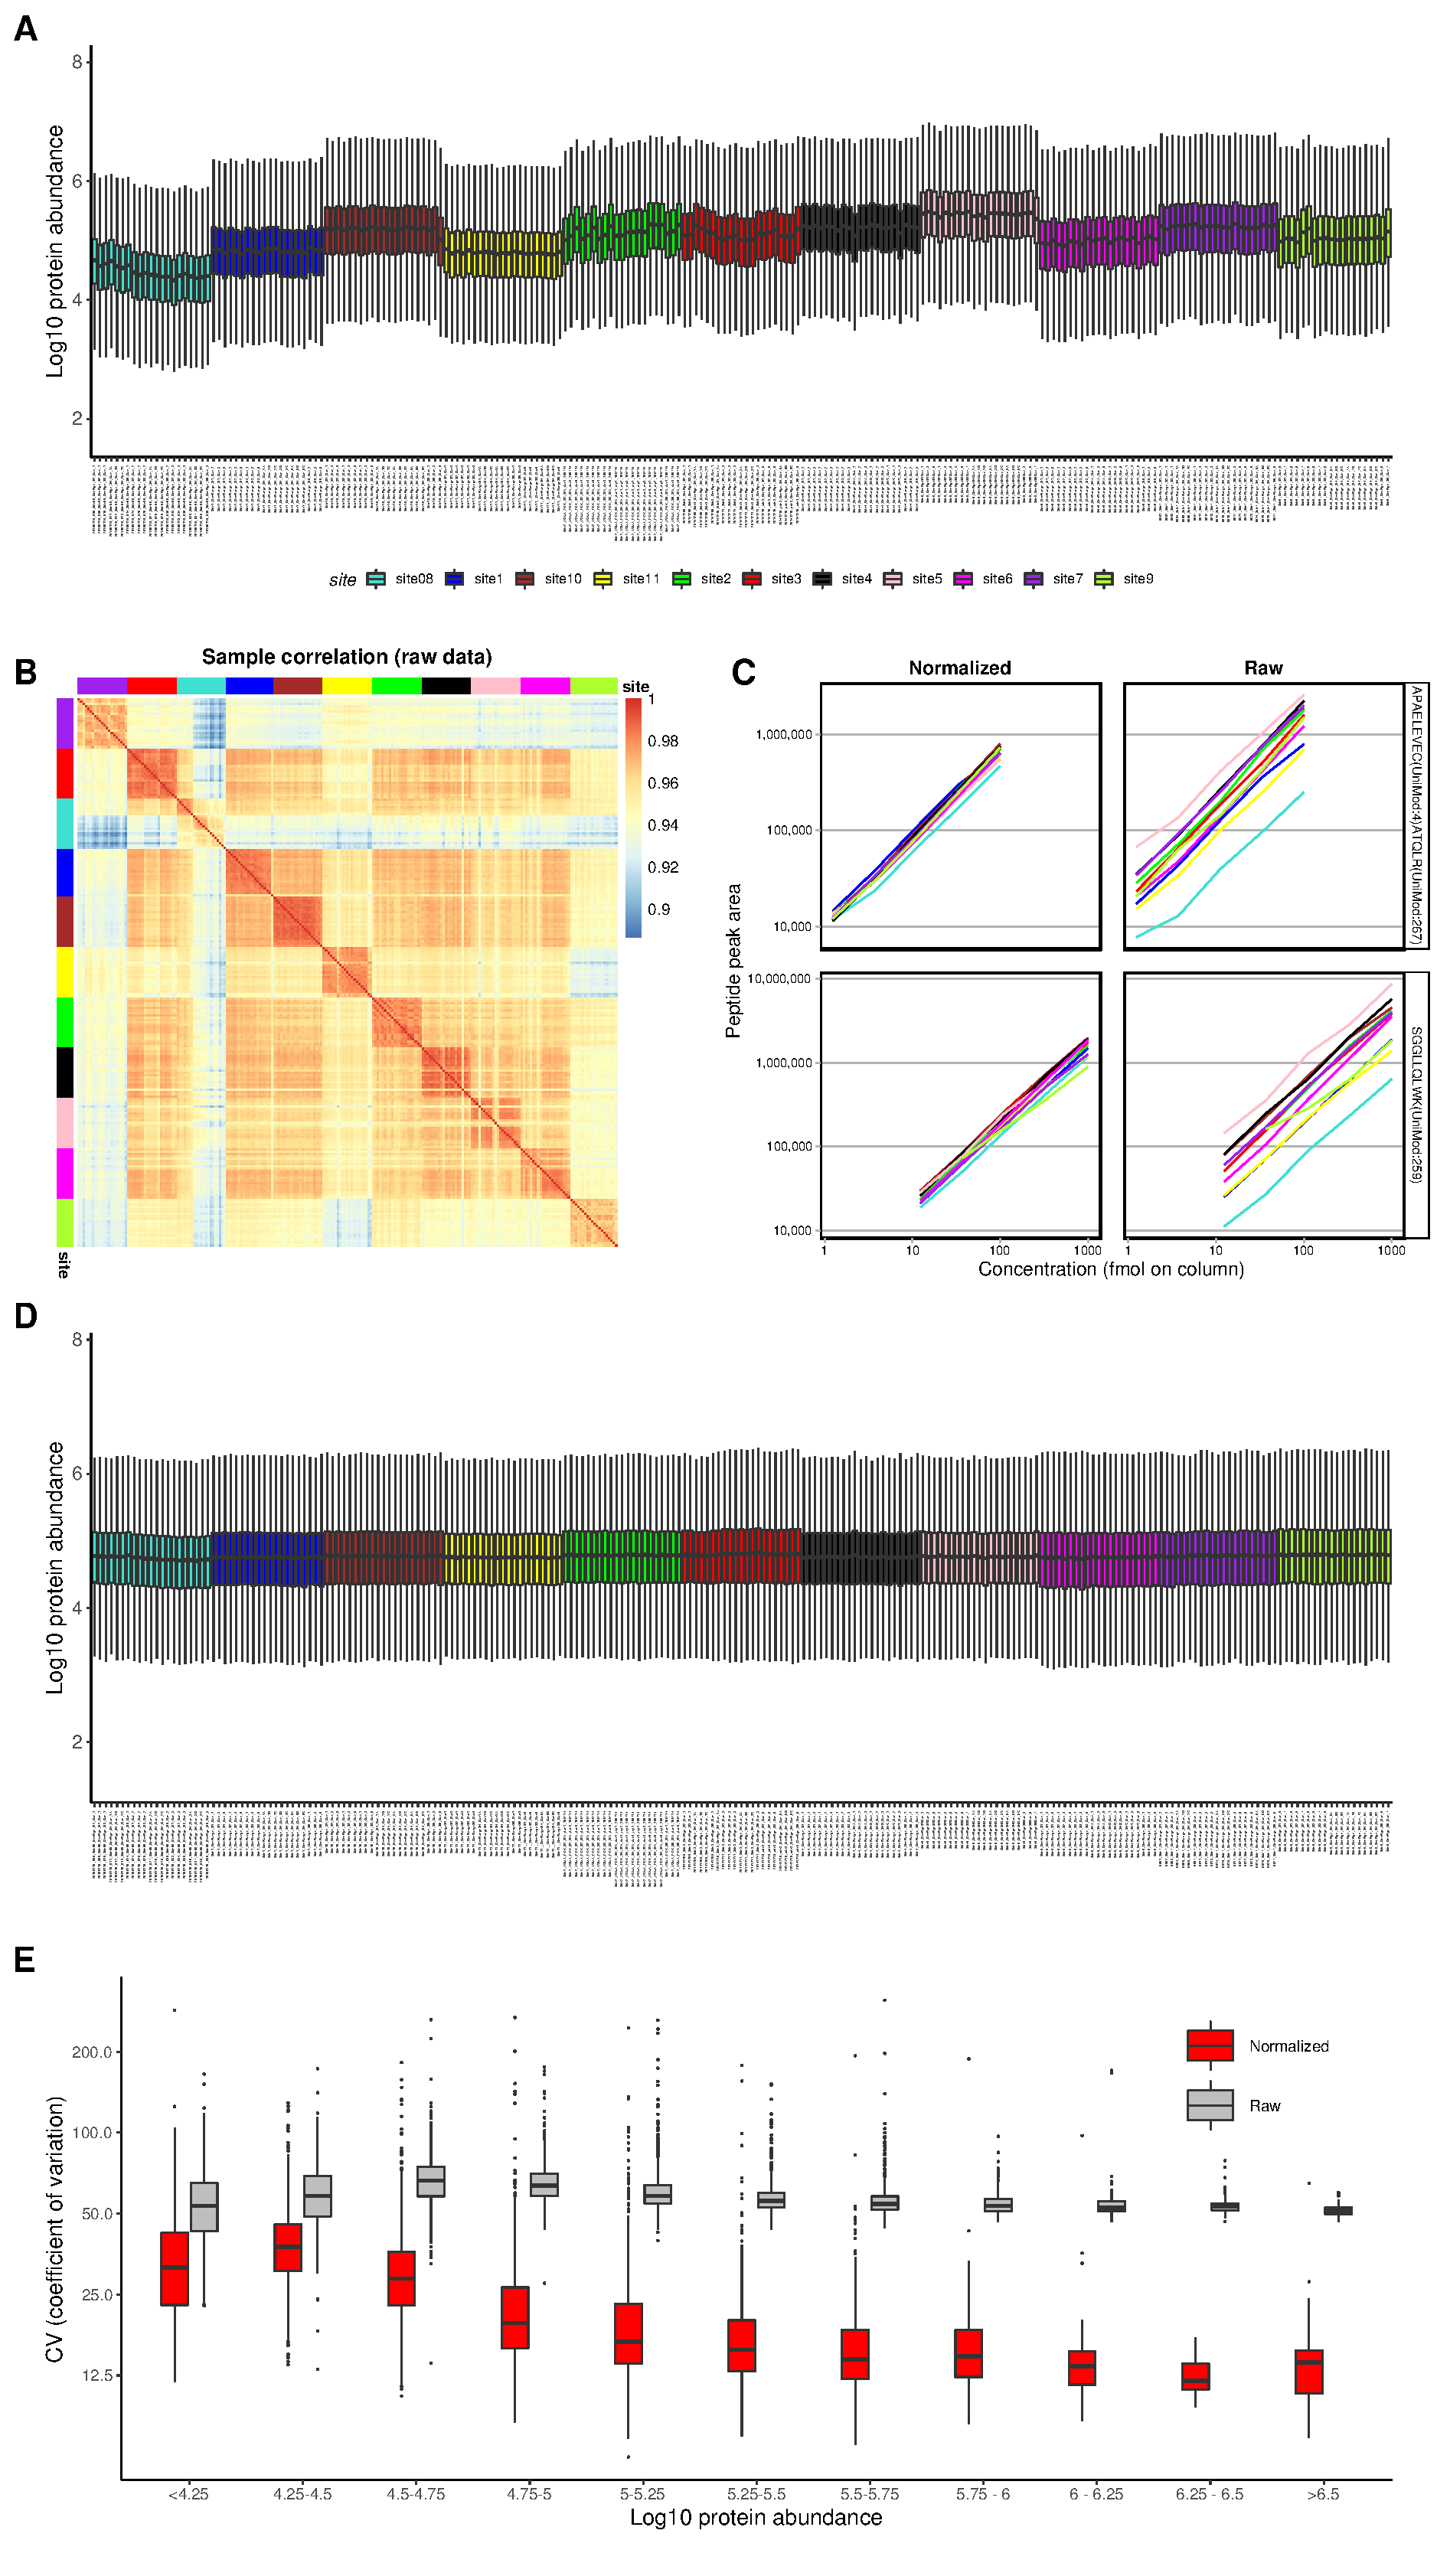
\includegraphics[width=\textwidth,height=.9\textheight,keepaspectratio]{figures/Supp_InterLab.pdf}
	\caption{\textbf{Batch effects in the InterLab study}\\
		 \footnotesize  (A) Boxplots of protein-level raw sample intensities colored by MS spectra acquisition sites (normalization on fragment-level); (B) Sample correlation heatmap, top row and left column colored by MS spectra acquisition sites, used as a quality control (protein-level data); (C) Comparison of two spike-in peptide quantification in raw and normalized data; (D) Boxplots of median-normalized sample intensities; (E) Quality control by comparing coefficient of variance (CV) for proteins, binned by log10 abundance.}
	\label{fig:batch_figS1_InterLab}
\end{figure}

\begin{figure}
	%\center
	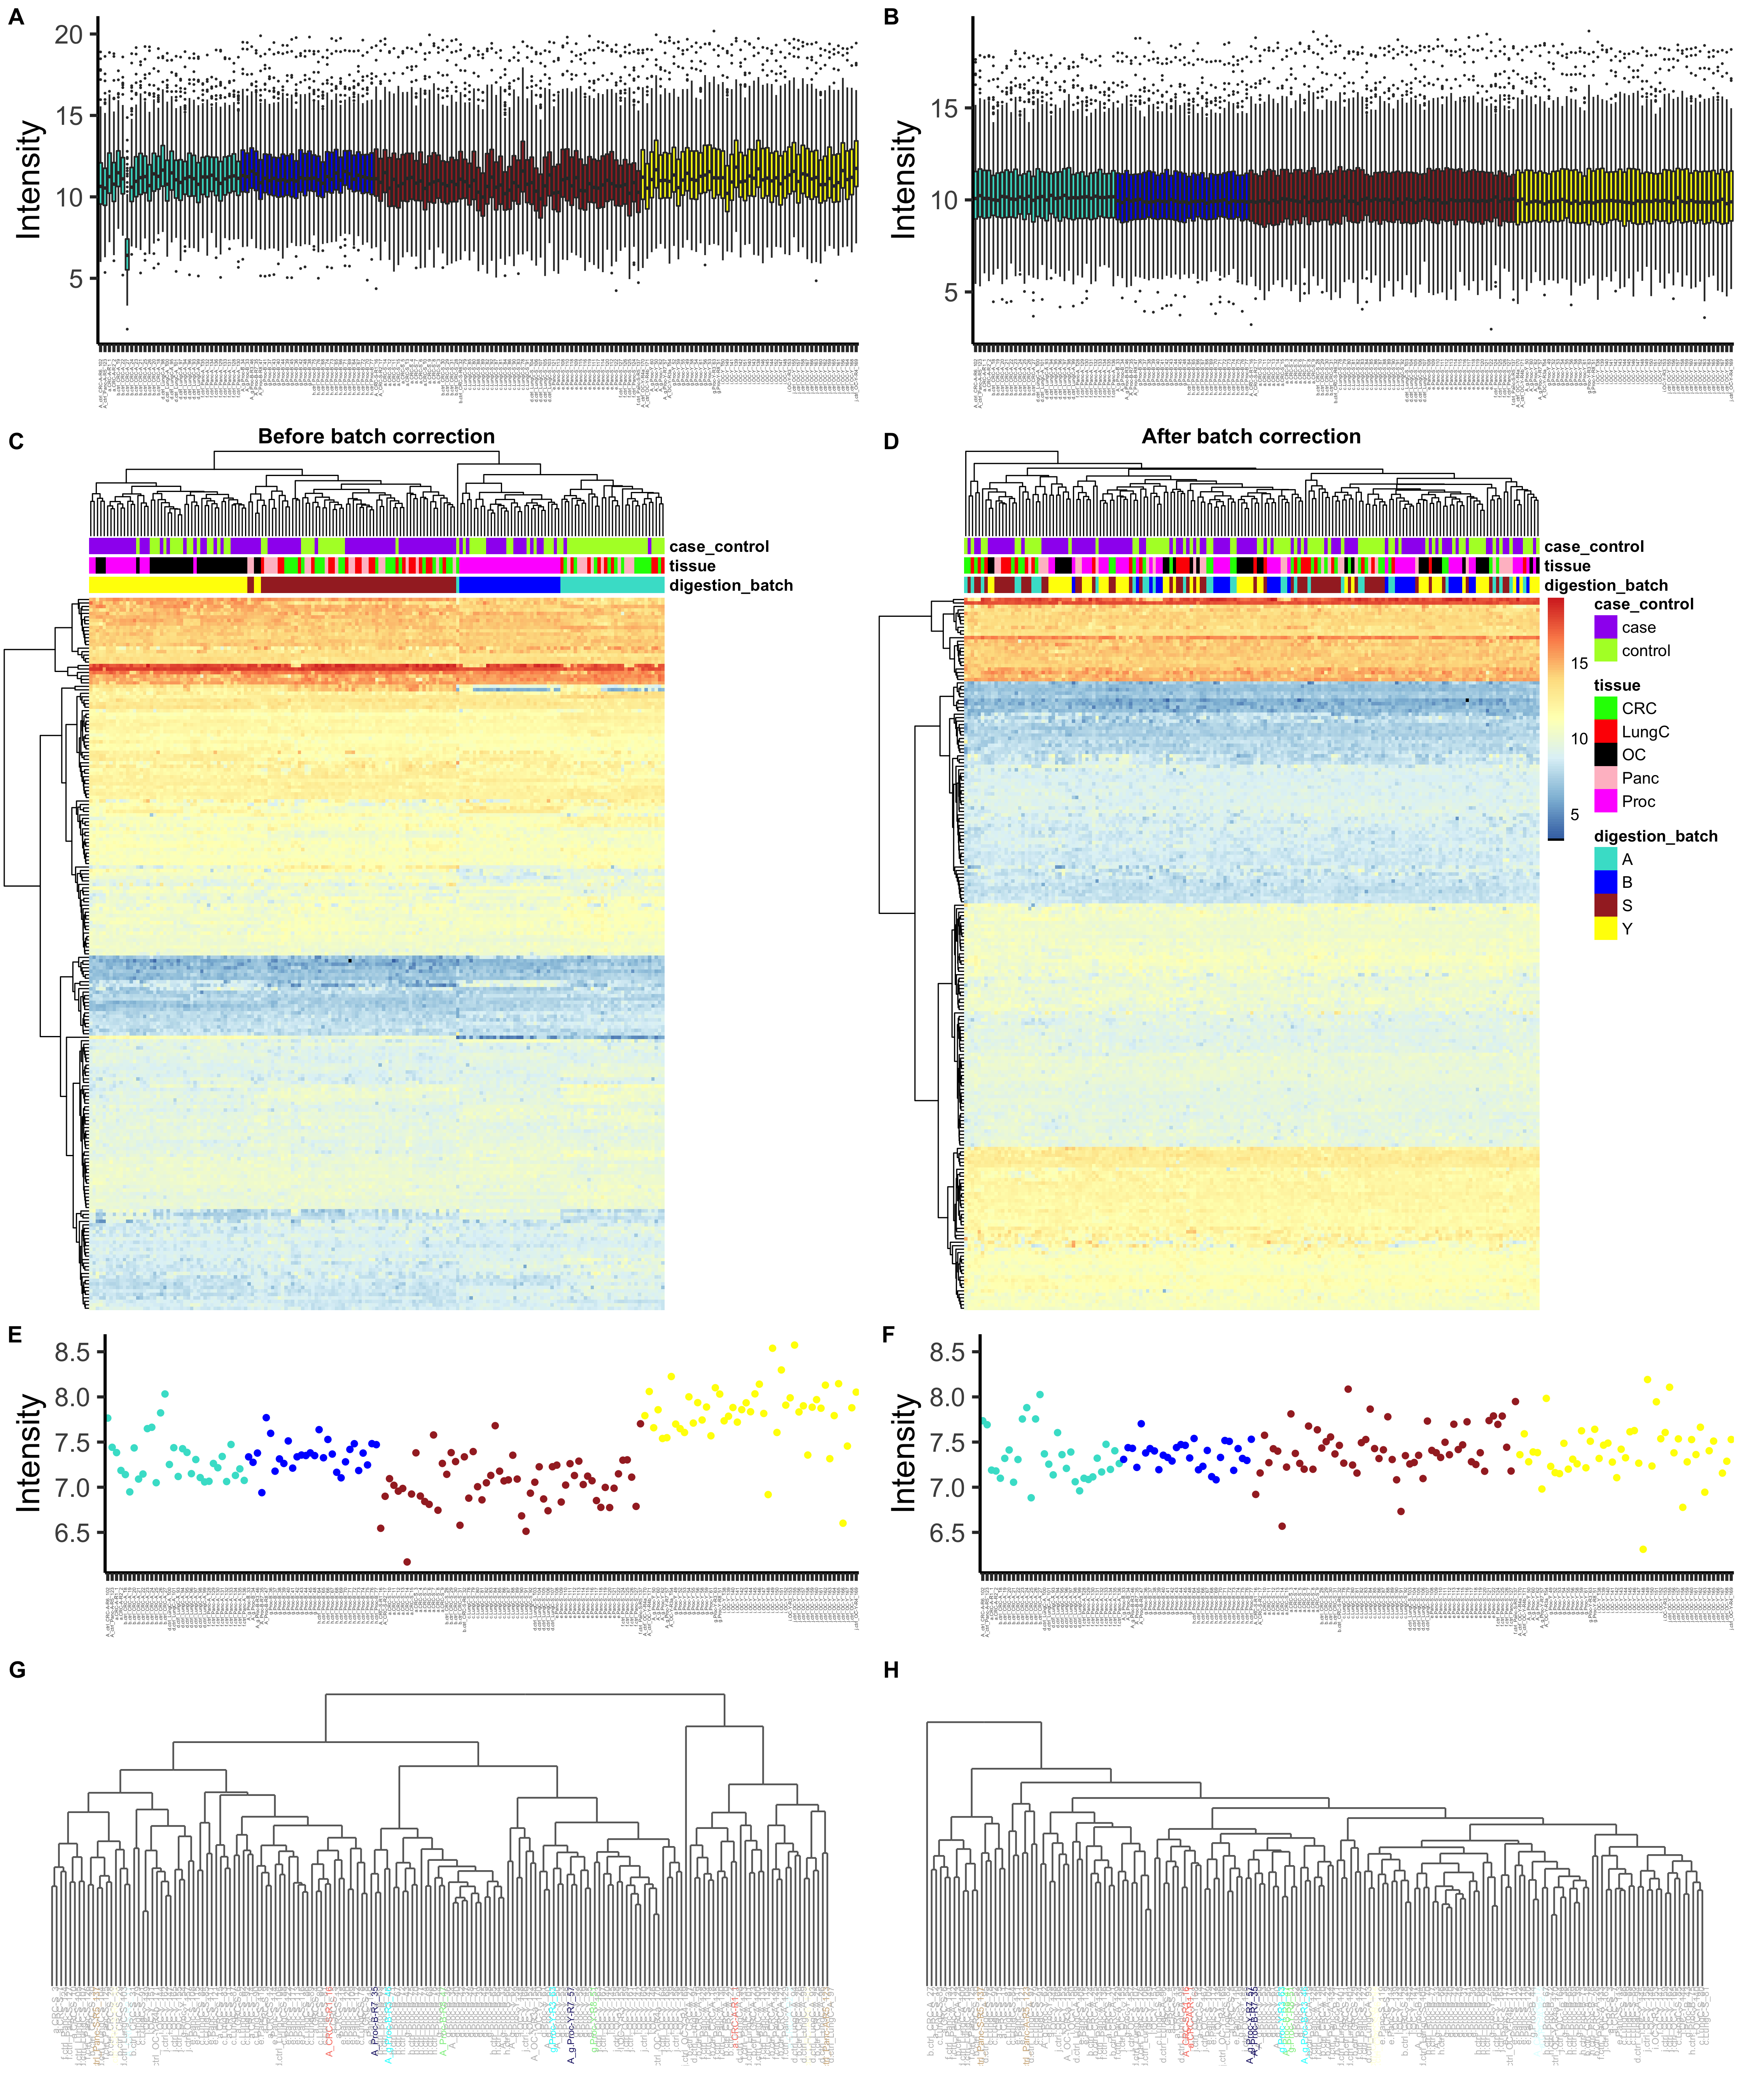
\includegraphics[width=\textwidth]{figures/Supp_Fig2_PanCancer.png}
	
	\caption{\textbf{Batch effects in the PanCancer study} \\
		\footnotesize (A) Boxplots of raw sample intensities colored by digestion batch; (B) Boxplots of normalized sample intensities colored by digestion batch; 
		(C) Hierarchical clustering and heatmap of raw protein-level data; (D) Hierarchical clustering and heatmap of batch corrected protein-level data; (E) Intensity of spike-in Fetuin in raw data; (F) Intensity of spike-in Fetuin in batch corrected data; (G) Hierarchical clustering of normalized data with Manhattan distance, with replicated samples colored; (H) Hierarchical clustering of batch corrected data with Manhattan distance, with replicated samples colored. All plots represent protein level data.}
	\label{fig:batch_figS2_PanCancer}
\end{figure}

\begin{figure}
	%\center
	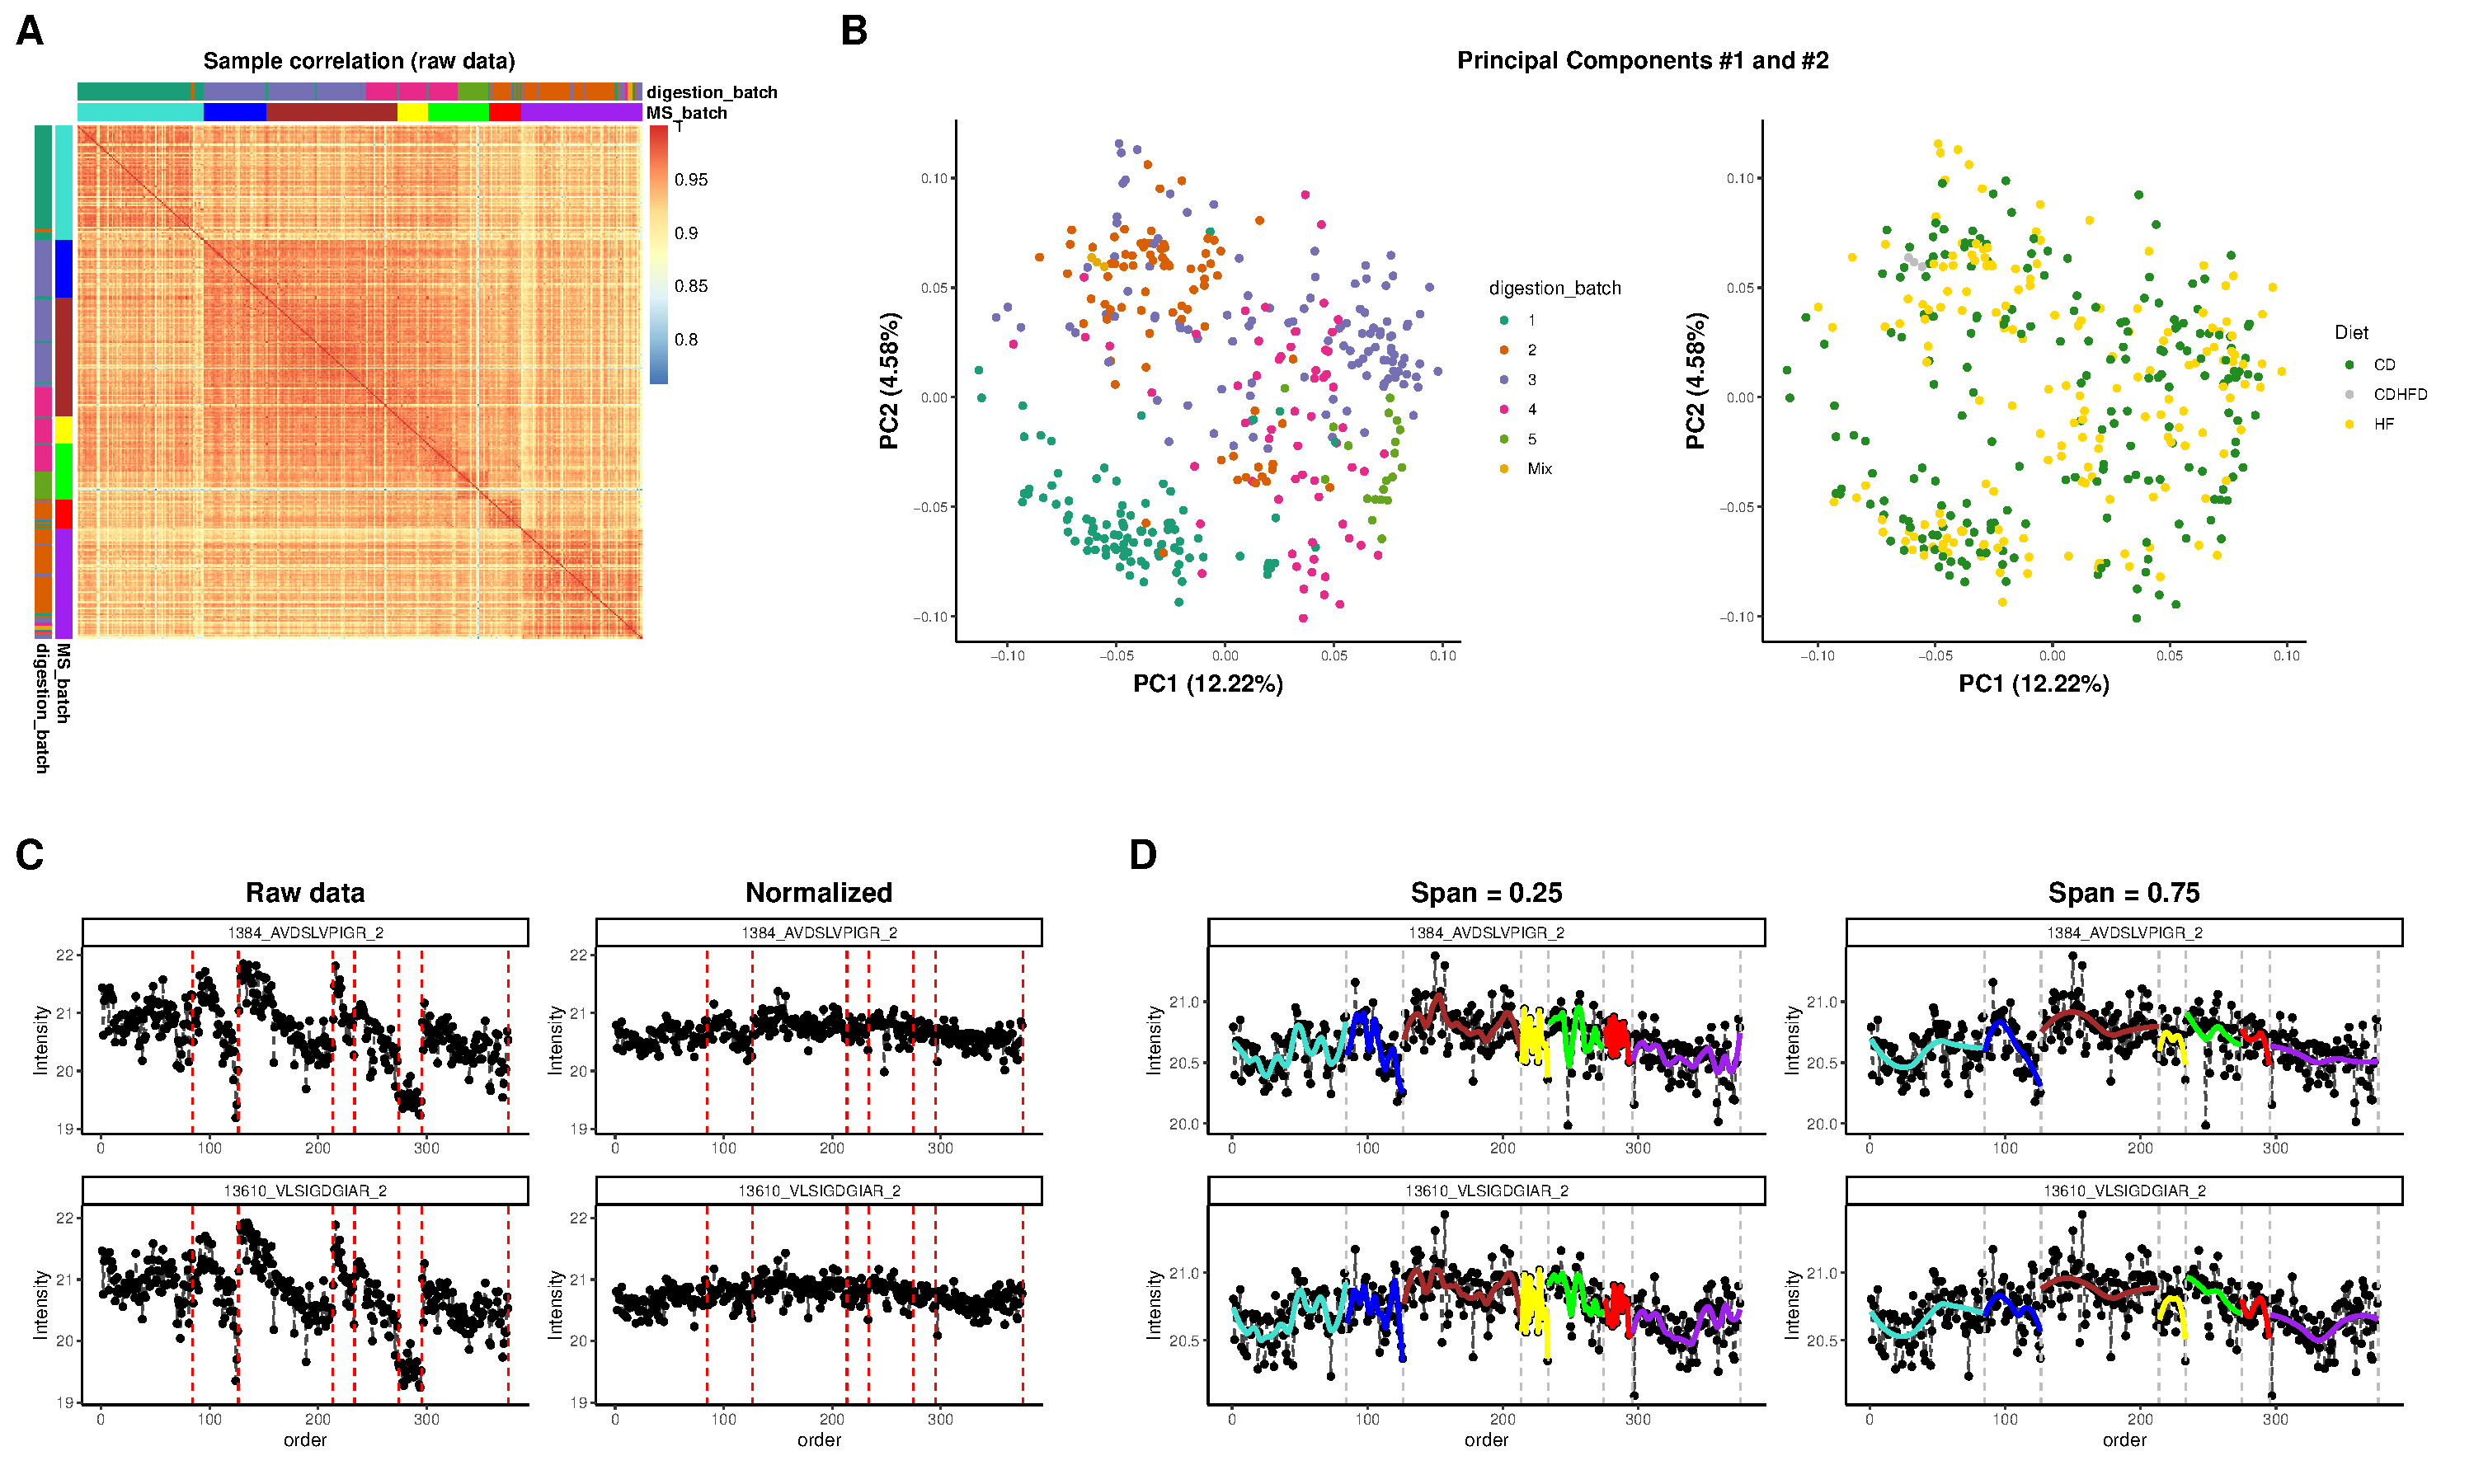
\includegraphics[width=\textwidth]{figures/SuppFig3_pipeline_extras.pdf}
	
	\caption{\textbf{Additional details of the pipeline} \\
		\footnotesize (A) Correlation of sample intensities indicates closer relationship between samples from the same batch; (B) Principal Components colored by digestion batch cluster together, but not the samples of mice on the same diet; (C) Normalization removes a large fraction of variation, making samples more comparable, this is also seen at the level of individual peptides; (D) Span has to be chosen carefully: when too small, it will lead to overfitting and overcorrection}
	\label{fig:batch_figS3_pipeline_extra}
\end{figure}


\begin{figure}
	%\center
	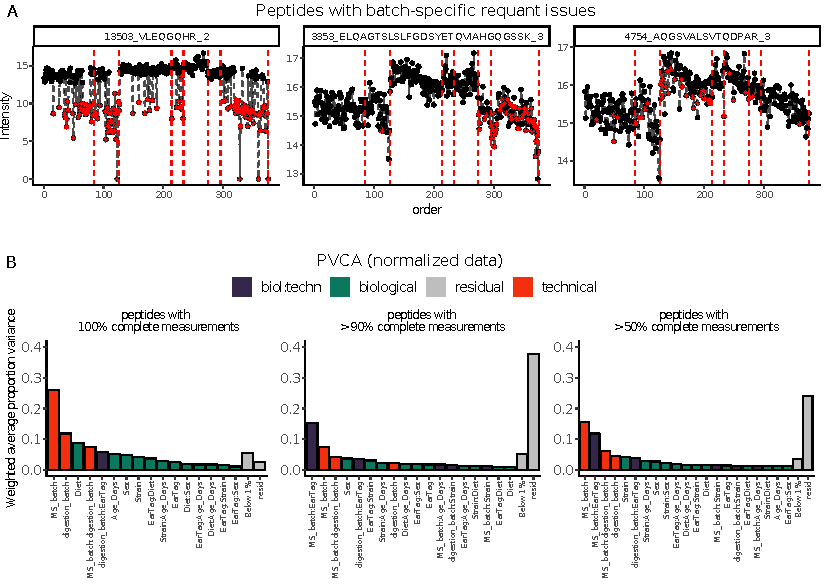
\includegraphics[width=\textwidth]{figures/Supp_Fig4_missing_values_extra.pdf}
	
	\caption{\textbf{Missing values and batch effects} \\
		\footnotesize (A) Re-quantification of elution traces can pick up batch-specific noise, that can be drastically different from confidently identified peptide fragments (left) or indistinguishable from those, meaning that values inferred should be treated with extreme caution; (B) PVCA can only be applied to complete matrices and thus missing values need to be inferred. This makes this method highly sensitive to missing values inference (here filled with 0). Depending on the completeness cutoff, variance distribution across technical and biological factors varies substantially. Note that when peptides with missing values are used in the analysis (panels center and right), a substantial portion of variance is attributed to "resid" (residual), meaning that this variance cannot be associated with any of known factors, indicating that missing value distribution is at least partially random.}
	\label{fig:batch_figS4_missing_values}
\end{figure}

\end{document}
